




\begin{comment}
MAIN REFS

DAYAL\&FERRARA , BARKANA\&LOEB, 

LONGAIR?, 


SUMMARY

 1. THE BIG PICTURE (A BRIEF HISTORY OF THE UNIVERSE, IE WHY WE ARE TALKING ABOUT ALL OF THIS) (INTRO BARKANA)
 
 2. THE FIRST STRUCTURES (LINEAR GROWTH OF PERTURBATIONS \& NON LINEAR COLLAPSE) (CAP 3 DAYAL)
 
 3. DM HALOS PROFILE
 
 4. GALAXIES AND FIRST STRUCTURES FROM LINE COOLING; 
 
 5. BASICS OF GAL FORMATION PHYSICS (ACCRETION, OUTFLOWS, IMF)
 
 6. COSMOLOGICAL SIMULATIONS;
 ZOOM IN IN HIGH REDSHIFT GALAXIES
 
 THINGS THAT IS USEFUL TO MENTION:
  - NFW
  - COOLING FUNCTION AND COOLING OF SPECIES 
  - UV BACKGROUND
  - ESCAPE FRACTION AND REIONIZATION
  - CGM ENRICHMENT/METALLICITY?
  - PRISTINE INFLOW AND OUTFLOWS
  - IMF AND POPULATION SYNTHESIS MODELS
  


-------

THINGS I COULD ADD:

 -  THERMAL HISTORY OF THE UNIVERSE
 - EXCURSION SET THEORY


-------
HISTORICAL INTRO ON GALAXY FORMATION (GALAXIES AS ISLES ETC)

DESCARTES AND GALAXIES AS UNIVERSE ISLES, HUBBLE AND THE BIRTH OF EXTRAGALACTIC ASTRONOMY (ANDROMEDA GALAXY)

TODAY THE PARADIGM HAS SHIFTED SIGNIFICANTLY --> MORE REALISTIC PICTURE WITH GALAXIES INTERACTING, ACCRETING, ETC

BRIEF DESCRIPTION OF THE CHAPTER -- STARTING WITH AN INTRODUCTION ON THE LCDM MODEL AND ITS PREDICITONS IN THE FIELD OF STRUCTURE FORMATION, WE WILL THEN REVIEW THE CURRENT PARADYGM IN GALAXY FORMATION AND WE WILL HIGHLIGHT THE ROLE OF DIFFERENT PHYSICAL PROCESSES WE WILL USE LATER ON IN THE DEVELOPMENT OF OUR WORK; 

(WE WILL LAY DOWN THE BASIS ...)



\end{comment}


In 1924, Edwin Hubble used the period-luminosity relation for Cepheid variables (discovered a decade before by Henrietta Leavitt) to prove that the Andromeda Nebula is a distant extragalactic system. This work posed an end, once and for all, to \textit{The Great Debate} in astrophysics: the universe we live in does not consist only of the Milky Way (MW), but in fact, it contains other galaxies similar to the one we live in. This milestone marked the beginning of extragalactic astrophysics.

\vspace{6pt}

Almost a century later, we are able to fully realize the vastness and the richness of the observable universe: the galaxies it contains are thought to be hundreds of billions. We have now the capabilities to observe many of them, starting from their infancy and following their growth and evolution through cosmic time. We have come up with a picture that is quite different from the idea of galaxies as "island universes" popularized by Immanuel Kant in the XVIII century: galaxies are not immutable and isolated objects that emerge from the cosmic void like islands in the ocean. Instead, they are giant open ecosystems, that form structures at different scales and are profoundly interconnected. Their evolution depends strongly on the influence of the external environment as well as on the interaction with neighboring objects. Since recent times, we have been able to disentangle this complex interplay and to identify some of the key factors that drive galaxies in their formation and evolution from the origin of the universe to our epoch. In this chapter, we review the recent advancements in this field: our goal is to inscribe the work developed in subsequent chapters inside a more vast and coherent framework.

\vspace{6pt}

In section \ref{sec:intro_cosmo}, we briefly introduce the standard model for cosmology. In particular, we focus on how structure formed under the influence of gravity, in the originally homogeneous universe, and on how they shaped the universe into the complexity of morphologies and compositions we observe today. In particular, we focus on the formation of dark matter halos: these objects are thought to be the key ingredients for the process of galaxy formation. Section \ref{sec:birth_galaxies} is devoted to the formation of the first stars and galaxies, as well as to their direct influence on the primordial universe. Finally, in section \ref{sec:physics_galaxies}, we explore the physical processes that regulate the evolution of these galaxies, laying down the bases and motivations for the topics we will discuss in the following chapters. We mainly follow the book written by T. Padmanabhan \citep{padmanabhan_book}, as well as the reviews by Barkana \& Loeb \citep{Barkana:2000fd}, Dayal \& Ferrara \citep{Dayal:2018hft}, and Sommerville \& Davé \citep{somerville2015physical}.

\section{A quick look at the big picture} \label{sec:intro_cosmo}
 
 \subsection{The $\Lambda$CDM model}
 
 In the last few decades, astounding progress has been made in improving our understanding of how the universe formed and evolved. Even though many questions remain open, we have developed what is now considered a standard paradigm for cosmology, the so-called $\Lambda \mathrm{CDM}$ (\textit{Lambda Cold Dark Matter}) model. This model founds on Einstein's General Relativity and on the "cosmological principle" to describe the evolution of the universe from its infancy until its end. This latter principle states that the distribution of matter and energy in the universe is isotropic on large scales. 
 
 Assuming the cosmological principle, it follows that the metric that describes the space-time of the universe must respect some particular symmetries, and it can be expressed in the form known as the FLRW (Friedmann-Leimatre-Robertson-Walker) metric:
 \begin{equation}
     \d s^2 = \d t^2 -a^2(t)\left(\frac{\d r^2}{1-kr^2} + r^2 \left(\d \theta^2 + \sin^2\theta \d \varphi^2\right)\right),
 \end{equation}
 where $a(t)$ is a global scale factor which describes how the universe expands with time, and $(r,\theta,\varphi)$ are comoving spherical coordinates. Note that the distance between two points in these coordinates is independent of time, while the physical distance $d(t)$ can be expressed in these coordinates simply as $d(t)=a(t)x$ (where $x$ is the comoving distance between the points). The constant $k$ stands for the sign of the spatial curvature: it is $+1$ in a \textit{closed} (spherical) universe, zero in a \textit{flat} universe, and $-1$ in an \textit{open} (hyperbolic) universe.
 
 
 %From simple arguments, the fact that the universe is expanding, as $a(t)$ increases with time, can be deduced: the physical distance bewtween us and another object can be expressed using the comoving coordinates $\mathbf{x}$ as $\mathbf{r}(t) = a(t) \mathbf{x}$. The physical velocity $\mathbf{v} = \Dot{\mathbf{r}}(t)$ can be expressed as $\mathbf{v} = H(t)\mathbf{r}=(\Dot{a}(t)/a(t))\mathbf{r}$.
 


 With this choice for the metric, Einstein equations can be recast into two equations, known as \textit{Friedmann equations} from the Russian physicist Alexander Friedmann. The first yields the relationship between the scale factor $a(t)$ and the energy content of the universe $\rho(t)$:
 \begin{equation}
     H^2(t) = \frac{\Dot{a}^2}{a^2} = \frac{8\pi}{3}G\rho - \frac{k}{a^2}
 \end{equation}
 The second equation is usually obtained considering the conservation of the stress-energy tensor. For a perfect fluid with
 an equation of state $P=P(\rho)$, this equation recalls the first principle of thermodynamics:
 \begin{equation}
     \Dot{\rho} + 3H(t)(\rho+P)=0
 \end{equation}
 Given a multi-component fluid, the total energy density is the sum of the different components, with each component scaling according to its own conservation law. The universe can in fact be considered as a multi-component fluid, with all the different fluids being described by an equation of state of the form $P=w\rho$: \textit{matter} has negligible pressure ($w=0$), because it is non-relativistic; \textit{radiation}, on the other hand, has $w=1/3$; the cosmological constant $\Lambda$ can be considered effectively as a fluid with $w=-1$ (this fluid is also called \textit{dark energy} to include hypothetical contributions different from the cosmological constant). With these definitions, the two Friedmann equations can be cast together in a very simple form by defining the critical density as:
 \begin{equation}
     \rho_c(t) = \frac{3H^2(t)}{8\pi G} \label{eq:friedmann_1}
 \end{equation}
 Using the critical density, we can define the dimensionless parameters for the different fluids:
 \begin{equation}
     \Omega_i (t)= \rho_i(t)/\rho_c(t)
 \end{equation}
 With $\Omega_m$, $\Omega_r$, and $\Omega_\Lambda$ denoting the present-day values of the quantity $\Omega(t)$ for matter, radiation, and dark energy respectively, the resulting equation reads:
 \begin{equation}
     H^2(t)= H_0^2\left(\Omega_m (1+z)^{3} + \Omega_r (1+z)^{4} + \Omega_\Lambda + \Omega_k (1+z)^2\right), \label{eq:friedmann_3}
 \end{equation}
 where we have also used the fundamental relation for cosmological redshift:
 \begin{equation}
     a^{-1}(t)=1+z(t)
 \end{equation}
 The parameter $\Omega_k$ accounts for the effect of curvature in the first Friedmann equation, and it is defined as:
 \begin{equation}
     \Omega_k = -\frac{k}{H_0^2} = 1-\Omega_m-\Omega_r-\Omega_\Lambda
 \end{equation}
 This equation can be solved to find the evolution of the scale factor $a(t)$ (or, equivalently, the redshift $z(t)$) with time. In order to do that, the values of the parameters $h$ (defined as $H_0=h100\, \,\kms\mathrm{Mpc}^{-1}$), $\Omega_m$, $\Omega_r$, $\Omega_\Lambda$ need to be obtained. 
 
 One of the most important achievements of the last decades of research in cosmology is the precise measurements of these parameters: the best estimate we have so far come from the Planck mission \citep{2016planck}, and it yields $h = 0.678\pm 0.009$, $\Omega_m = 0.3156 \pm 0.0091$ and $\Omega_\Lambda =  0.6844 \pm 0.0091$, $|\Omega_k < 0.005|$.
 The matter parameter $\Omega_m$ is composed of two different components: baryons (ordinary matter) and \textit{dark matter} (DM). They contribute to the energy budget with their respective parameters as $\Omega_b = 0.0492 ± 0.0002$, $\Omega_{DM} = 0.2647 \pm 0.0003$ \citep{2016planck}. Dark matter is a type of matter which differs from ordinary baryonic matter because it does not interact with light and thus it is not directly observable. Nevertheless, its existence is supported by many indirect evidences, and - as it will become clear in the next section - the $\Lambda \mathrm{CDM}$ poses its foundations on the existence of this matter component ($``\mathrm{CDM}"$ stands for \textit{Cold Dark Matter}).
 
 Overall, the value of the parameters describe a flat universe that is expanding with time (the physical distance between two points increases as $a(t)$ increases), and whose expansion is in fact accelerating because of the presence of the $\Lambda$ term: the future of the universe -- according to these parameters -- will be dominated by this acceleration term, and the scale factor $a(t)$ will continue to increase indefinitely with a rate close to an exponential behavior.
 
 As for the past evolution of the universe, we can describe the cosmic history by imagining to reverse the expansion we witness today: in this way, we get a universe that becomes smaller and denser as time decreases. Taking the limit as time goes to zero, we find that the universe started at a point of infinite density and temperature: this is known as the \textit{Hot Big Bang theory}. According to this theory, the environment that characterizes the primordial universe is so dense and hot that the frequency of collisions and reactions between the different species guarantees the presence of thermodynamical equilibrium. As the universe expands, its temperature decreases adiabatically, because equilibrium is instantly restored. When the rate of expansion gets larger than the rate of collisions for a given species, however, that species decouples from the thermal bath and travels freely (i.e. with no interactions) as a relic of the primordial universe.  
 
 \begin{figure}
	\centering
	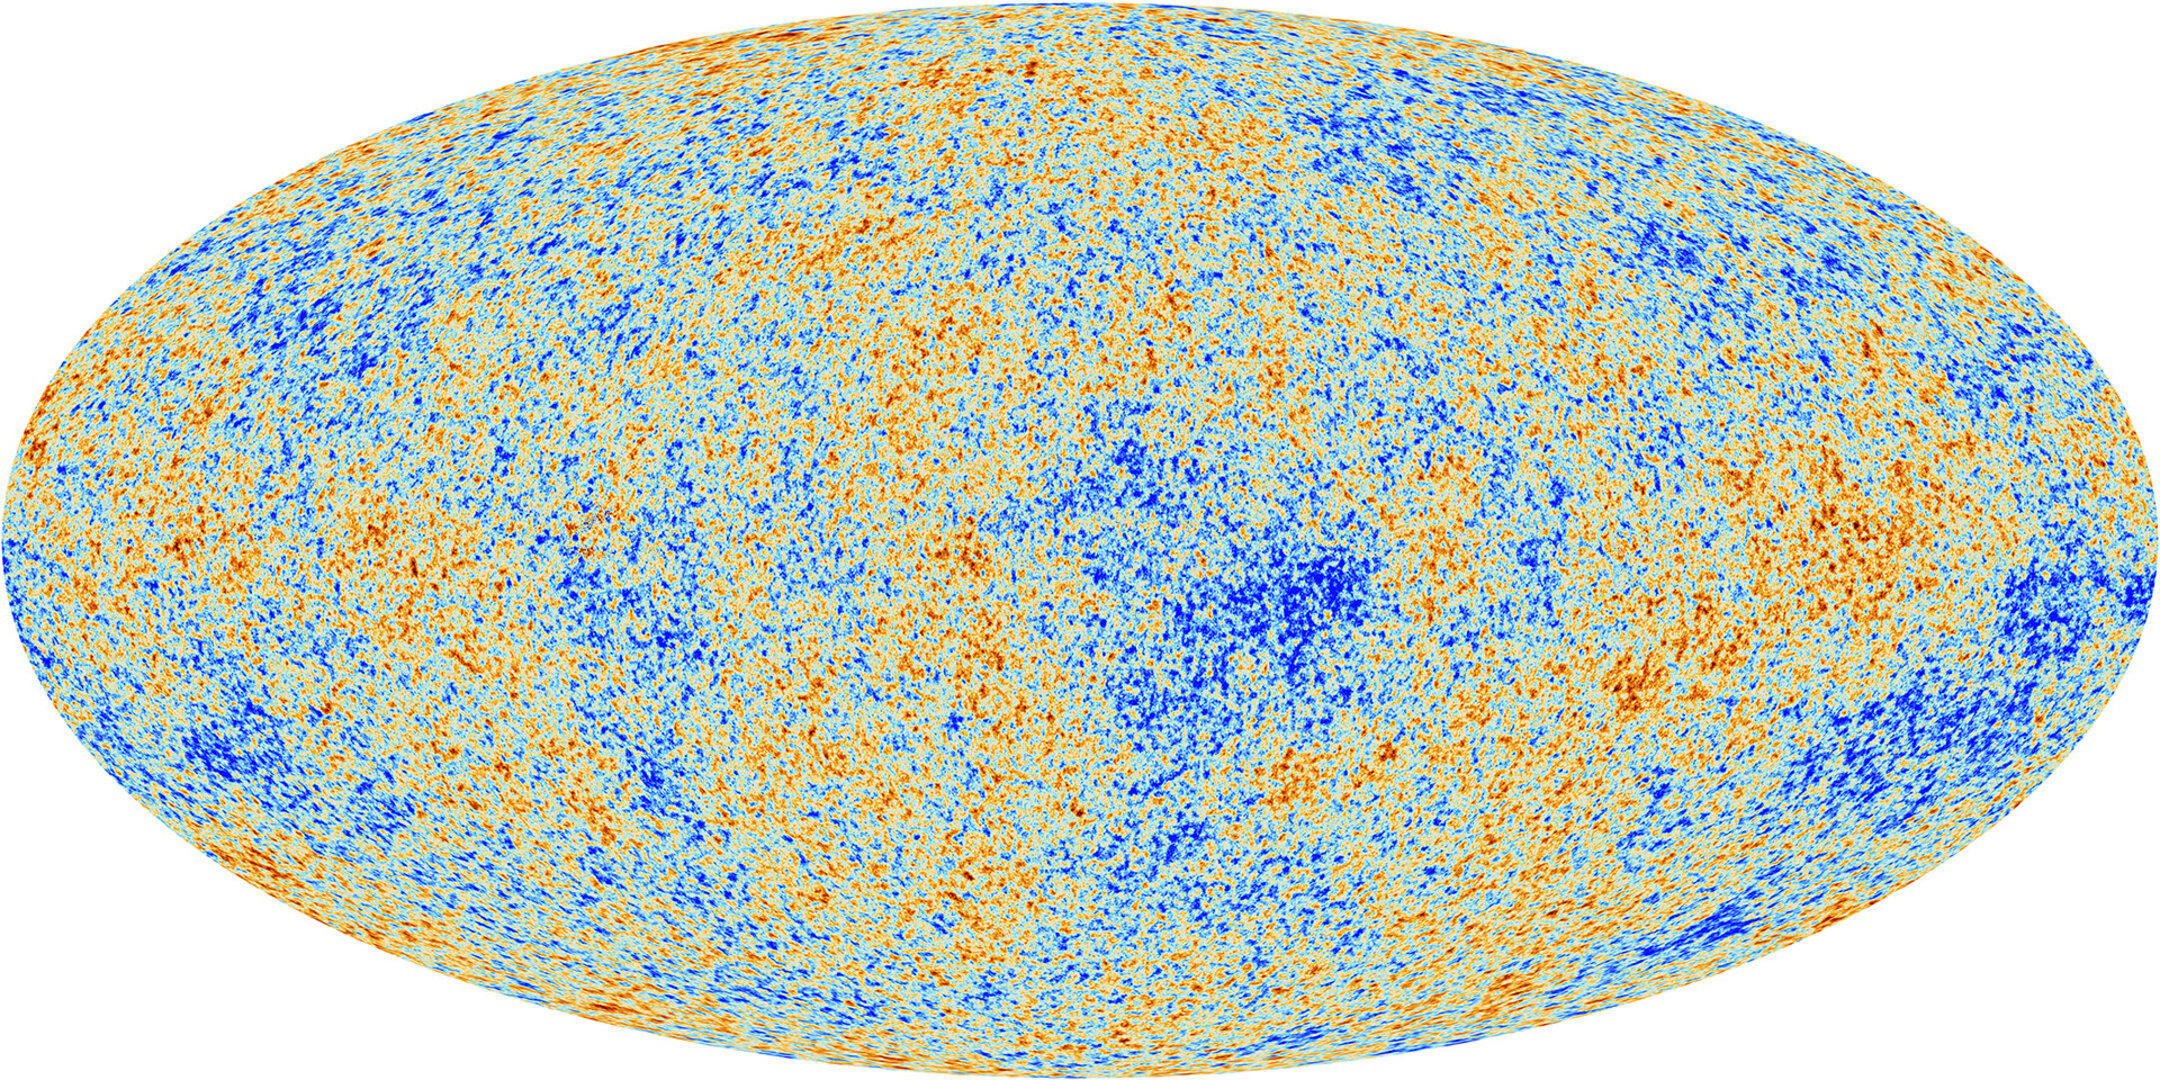
\includegraphics[width=1.\textwidth]{plots/Planck_CMB_pillars.jpg}
	\caption{Temperature fluctuations (on the scale of $10^{-5}$) of the Cosmic Microwave Background, as observed by the ESA Planck mission \citep{2016planck}.  
	}
	\label{fig:CMB}
\end{figure}


 The \textit{Cosmic Microwave Background} (CMB), discovered by Penzias and Wilson in 1965 \citep{penzias_wilson_cmb}, is the most important instance of these relics: photons decouple from the other species around 300.000 years after the Big Bang, in a process known as \textit{last scattering}, and offer us an imprint of the physical conditions of the primordial universe. The energy distribution of the CMB photons is shaped like a black body (Planck distribution):
 \begin{equation}
     I(\nu;T) = B_\nu(T) =  \frac{2h}{c^2} \frac{\nu^3}{e^{(h\nu/kT)}-1} \label{eq:black_body}
 \end{equation}
 This is expected since photons at decoupling are in thermal equilibrium, and the form of their distribution does not change as the universe expands. The temperature $T$ is strikingly uniform in the different regions of the sky: this is a strong hint in favor of the cosmological principle. However, small fluctuations at the level of $10^{-5}$ were found in the temperature distribution by the NASA COBE mission in 1992 and later described with more detail by the WMAP and Planck missions (figure \ref{fig:CMB}). These small fluctuations are one of the most important features of observational cosmology: they are considered to be the first seeds that are destined to grow into the structures we observe today in our universe. Stars, black holes, galaxies, clusters of galaxies, filaments: all of the features of the rich and complex universe we live in are thought to be originated from these small perturbations of the Cosmic Microwave Backgrounds. In the next few sections, we will explore how these perturbations grew under the influence of gravity, and eventually led to the formation of galaxies and the large-scale structure observed in the present universe.
 
 

 \subsection{Linear structure formation}
 
 The origin of the perturbations we observe in the CMB spectrum is still a matter of debate. The most reasonable and widely accepted explanation comes from the theory of \textit{cosmic inflation}. According to this theory, the universe underwent a \textit{quasi De-Sitter} phase of expansion early after the Big Bang. During this phase, quantum perturbations of the field that drove the inflationary process are turned into classical perturbations of the metric and the energy density of the universe. These classical fluctuations are directly related to the ones we measure the temperature spectrum of the CMB. 
 
 Despite the success of an inflationary mechanism in explaining many unsolved problems in cosmology, there is still no consensus on the mechanism that made the Universe inflate. Moreover, observational evidences are still lacking, allowing only a few constraints on the inflationary parameters and ruling out only a small part of the proposed models. Here, we do not investigate the inflationary theories any deeper: we assume that -- in accordance with CMB observations -- some fluctuations are present in the spatial distribution of the energy density. Our goal is to consider these perturbations as initial conditions and to study their evolution in the expanding universe. We will consider comoving coordinates, and work with the density contrast:
 \begin{equation}
    \delta(\mathbf{x}, t) = \frac{\rho(\mathbf{x},t)}{\Bar{\rho}(t)} -1 = \frac{n(\mathbf{x},t)}{\Bar{n}(t)} -1 ,
 \end{equation}
 where the quantity $\Bar{\rho}(t)$ represents the background energy density at time $t$ ($n$ stands for the numerical density).
 
 The correct way to proceed would be to consider the Einstein equations and to perform the linearization of these equations to find the correct evolution of the perturbations in curved space-time. We choose to consider here the Newtonian approximation: we work with the equations of non-relativistic hydrodynamics, coupling them with the Poisson equation for gravity. This approach holds as long as the perturbations are small in intensity as well as in scale: if these hypotheses are true, the gravitational potential is weak enough to consider valid the Newtonian regime, and the effects of the curvature of space are completely negligible. The former assumption is always valid since we consider only the regime where perturbations are small; the latter is shakier since large-scale perturbations play a relevant role in our discussion. For our purposes, it will suffice to know that the results in the Newtonian case and in the general relativistic one are completely equivalent \citep[for more details, see][]{chisari2011connection}.
 
 The hydrodynamics equations (continuity and Euler equations) for a fluid in an expanding universe in comoving coordinates $\mathbf{x}$, and subjected to the influence of a gravitational potential $\varphi(\mathbf{x})$ are ($\mathbf{v}=a\mathbf{x}$ is the peculiar velocity):
 \begin{subequations}
 \begin{align}
    \frac{\partial n}{\partial t} + 3Hn + \frac{1}{a}\mathbf{\nabla}\times(n\mathbf{v}) &= 0 \label{eq:mass_cons} \\
    a\left(\frac{\partial }{\partial t} + \frac{\mathbf{v}}{a}\times\mathbf{\nabla}\right)(Ha\mathbf{x}+\mathbf{v}) &= -\frac{1}{\rho}\mathbf{\nabla} P - \mathbf{\nabla}\varphi \label{eq:euler}
 \end{align} 
 \end{subequations}
 We have to consider also the Poisson equation for the gravitational potential, which in comoving coordinates reads:
 \begin{align}
 \mathbf{\nabla}^2 \varphi = 4\pi G \rho a^2 \label{eq:poisson}
 \end{align} 
 Expanding these relations and taking the first order of these equations in the density contrast $\delta(\mathbf{x},t)$, we are left with this system of equations:
 \begin{subequations}
 \begin{align}
    \Dot{\delta} &= - \frac{1}{a}\mathbf{\nabla}\times \mathbf{v}\label{eq:euler_linearized1}\\
    a(\Dot{\mathbf{v}}+H\mathbf{v}) &= -\frac{1}{\Bar{\rho}}\mathbf{\nabla}\delta P - \mathbf{\nabla}\delta\varphi\label{eq:euler_linearized2}\\
    \mathbf{\nabla}^2\delta\varphi &= 4\pi G\Bar{\rho}a^2\delta \label{eq:euler_linearized3}
 \end{align} 
 \end{subequations}
 The system is not closed unless we provide an equation of state for the fluid. So far, we have made no explicit assumptions on the fluid properties (however, if we were to consider radiation, the coupling between energy and the gravitational potential would be different). 
 
 At this point, however, the subtle difference between dark matter and baryons comes to play: since dark matter interacts neither with photons nor with itself -- any non-negligible self-interaction is excluded by experimental observations \citep{tulin2018dark} --, it has no pressure, hence we can completely neglect the pressure gradient term in the Euler equation (eq. \ref{eq:euler_linearized2}). Ordinary matter, on the other hand, is strongly coupled with photons until last-scattering, and it can also provide a pressure term if the temperature is not too low. This different behavior determines the fate of the two species: being pressureless, dark matter perturbations can grow under the influence of gravity without any force to oppose this growth, while ordinary matter has its own pressure -- and also the radiative pressure of photons, as long as they are coupled -- to counterbalance gravity. This means that dark matter perturbations will grow until they become non-linear well before baryonic perturbation can do the same. As soon as dark matter is sufficiently clumped, it forms gravitational wells that attract baryons. For this reason, in what follows, we analyze only the growth of dark matter perturbations. In section \ref{sec:birth_galaxies}, we will then consider baryons and analyze the competition between gravitational pull and pressure support that determines their evolution. 
 
 For a pressureless fluid, we can combine eqs. \ref{eq:euler_linearized1}--\ref{eq:euler_linearized3} in one single equation (for example, taking the time derivative of eq. \ref{eq:euler_linearized1} and the gradient of eq. \ref{eq:euler_linearized2}). We get:
 \begin{align}
    \Ddot{\delta} + 2H\Dot{\delta} = 4\pi G \Bar{\rho}\delta \label{eq:euler_growing_delta}
 \end{align}
 This is the equation of a (time-dependent) damped harmonic oscillator with an imaginary frequency. There are in general two independent solutions: a \textit{growing mode} increasing with time, and a decaying mode that does the opposite. Starting with random initial conditions, this growing mode comes to dominate the density evolution. Hence, until it becomes non-linear, the density perturbation maintains its shape in comoving coordinates and grows in proportion to a growth factor $D(t)$.
 The damping term contains the Hubble parameter, and it is therefore known as the "Hubble friction" term; it has the same role of friction in the sense that -- in comoving coordinates -- perturbations grow more slowly because of the expansion of the universe. The intensity of this damping depends on the time dependence of the Hubble factor. Tentatively, the faster the universe expands, the slower the perturbations grow with time. In turn, the expansion rate depends on the energy budget of the universe: when the universe is dominated by radiation, the scale factor is $a(t)\sim t^{1/2}$ (and therefore $H(t)=1/2t$); for a matter-dominated universe, instead, $a(t)\sim t^{2/3}$ ($H(t)=2/3t$). Since the relevant part of the growth of perturbations happens after the \textit{matter-radiation equality} (i.e., when matter took over the energy budget, approximately 100.000 years after the Big Bang), we will solve eq. \ref{eq:euler_growing_delta} using for $H(t)$ this latter dependence. 
 
 Substituting the term $4\pi G\Bar{\rho}$ in accordance with the first Friedmann equation (eq. \ref{eq:friedmann_3}) in a matter-dominated universe, eq. \ref{eq:euler_growing_delta} becomes:
 \begin{align}
    \Ddot{\delta} + \frac{4}{3t}\Dot{\delta} - \frac{2}{3t^2} \delta = 0
 \end{align}
 The growing solution can be found simply guessing a power-law solution in the form $\delta\sim t^n$:
 \begin{align}
    \delta(t) \sim D(t) \sim a \sim t^{2/3} \label{eq:growth_factor}
 \end{align}
 Therefore, perturbations will grow with this time factor until the linear approximation breaks down, and the full non-linear collapse must be followed (section \ref{sec:nonlinear_collapse}). 
 
 Note that the growth factor $D(t)$ does not depend on the scale of the perturbation: in a matter-dominated universe, small-scale and large-scale perturbations grow in the same way. This does hold in the first phase of the universe expansion, when radiation dominates over matter: because of the gravitational coupling between radiation and dark matter, \textit{super-horizon} perturbations (i.e., that have a size larger than the horizon $d_H(t) = cH^{-1}(t)$) behave differently than perturbations that are inside the horizon. For this reason, it is useful to analyze perturbations at fixed scale in the Fourier domain, defining a perturbation with scale $\mathbf{k}$ as:
 \begin{align}
    \delta_\mathbf{k}(t) = \int \d^3\mathbf{x}\, \delta(\mathbf{x},t) \,e^{-2\pi i \mathbf{k}\times\mathbf{x}}
 \end{align}
 Moreover, this approach is particularly useful as inflation theories predict perturbations given by a Gaussian random field, in which different $\mathbf{k}$-modes are statistically independent of each other. For this reason, the statistical properties of the perturbations can be described entirely by a quantity that is related to the variance of the perturbations with scale $\mathbf{k}$, known as the \textit{power spectrum} $P(\mathbf{k})$:
 \begin{align}
    \langle \delta_\mathbf{k} \delta^*_\mathbf{k'} \rangle = (2\pi)^3 \,P(k)\, \delta^{(3)}(\mathbf{k}-\mathbf{k'})
 \end{align}
 Note that the quantity $\delta^{(3)}$ is the three-dimensional Dirac delta function. According to standard models of inflation, primordial fluctuations in the energy density field have a power spectrum $P_0(k)$ following a power law of the form:
  \begin{align}
   P_0(k) \sim k^{n_s},  
  \end{align}
 where $n_s$ is determined by the inflationary parameters, but in all models it is a number close to unity (observations measure $n_s = 0.9645 \pm 0.0049$ \citep{2016planck}). 
 
 In the radiation-dominated epoch, the original inflationary power spectrum gets distorted by the different behavior of sub- and super-horizon perturbations. The resulting power spectrum is characterized by a turnover at scales of the order of the horizon at matter-radiation equality $cH^{-1}(t_\mathrm{eq})$: for larger scale, the original $k^{n_s}$ dependence is retained, while smaller scales are depressed with a factor $k^{n_s-4}$. As perturbations grow, the global amplitude of the power spectrum scales with the factor $D^2(t)$: the left panel of figure \ref{fig:power_spectrum} presents the power spectrum shape and its evolution with redshift according to the linear theory of growth. 
 
 The overall normalization factor, however, is a free parameter of the $\Lambda \mathrm{CDM}$ model, and it is usually expressed in terms of the variance of the smoothed power density field $\sigma^2(M)$. Considering the density perturbation smoothed at a scale $R$ (or equivalently at a mass $M=4\pi R^3 \Bar{\rho} /3$) has the practical purpose of determining the formation of objects at that particular scale. To apply the smoothing, we have to consider a window function $W(\mathbf{x})$: the most common choice is the spherical top-hat, for which $W=3/4\pi R^3 \Bar{\rho}$ in a sphere of radius $R$ and zero outside. With the choice of a window function, we can express the variance of density perturbations at a scale $M$ in terms of the power spectrum $P(k)$:
  \begin{align}
   \sigma^2(M) = \frac{1}{(2\pi)^2}\int \d k \, k^2\,P(k)\,\Tilde{W}(kR),  \label{eq:sigma_2_M}
  \end{align}
 where $\Tilde{W}(k)$ is the three-dimensional Fourier transform of the window function. In figure \ref{fig:power_spectrum} (right panel), we plot the variance $\sigma^2(M)$ as a function of the mass $M$ and the redshift $z$. From this plot, we can infer a fundamental property of structure formation in the $\Lambda \mathrm{CDM}$ model: since $\sigma^2(M)$ is monotonically decreasing with mass, the process of formation of collapsed structures is hierarchical (also known as "bottom-up"); first, smaller structures form out of regions where the density field is significantly larger than average, then these structures merge to form high-density regions even at larger scales. For this reason, in the next section, we will study in a simplified setting how a small-scale perturbation grows non-linear and collapses under the influence of gravity.
 
  \begin{figure}
	\centering
	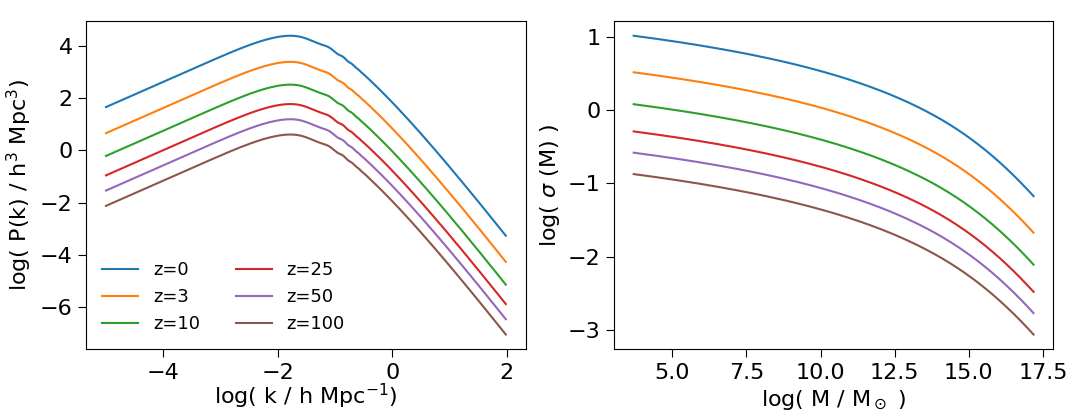
\includegraphics[width=1.0\textwidth]{plots/cosmo_1.png}
	\caption{\textit{Left}: power spectrum $P(k)$ at different redshifts $z$. At large scales (small $k$), the primordial $k^{n_s}$ dependence is retained, while at small scales (large $k$) the primordial dependence is tapered by a factor $k^{-4}$. Note that the growth with redshift is uniform in scale, as predicted by linear perturbation theory: non-linear effects such as halos formation and collapse are not considered. \textit{Right}: variance of the smoothed density perturbations at a mass scale $M$, for different redshifts $z$. The quantity $\sigma^2(M)$ can be obtained from the power spectrum $P(k)$ using eq. \ref{eq:sigma_2_M}.
	These plots were realized using the Python package \code{colossus} \citep{colossus2016}.}
	\label{fig:power_spectrum}
\end{figure}
 
 
 \subsection{Non-linear collapse} \label{sec:nonlinear_collapse}
 
 The linear approximation holds as long as perturbations are small ($\delta\ll1)$. However, perturbations are destined to leave the linear regime as they grow according to the factor $D(t)$. Describing the full, non-linear evolution of perturbations is extremely difficult: it is an N-body problem, where the gravitational interplay between all the different particles makes an analytical description of the time evolution not viable. The only general approach to the problem is to resort to numerical simulations: at every time step, the force acting on every particle is determined by computing the gravitational pull of all the other particles (usually in an approximated way). Hence, evolving every particle according to the equations of motion, the global evolution can be described with a good degree of accuracy. We will briefly elaborate on the capabilities of numerical simulations in section \ref{sec:physics_galaxies}.
 
 Here, we study the problem in a very simplified setting: we consider a matter-dominated universe, with a uniform background density $\Bar{\rho}(t)$. Within this background, we study the evolution of a single overdense blob with radius $R$ and uniform density $\rho (t) = \Bar{\rho}(t)(1+\delta(t))$. Clearly, the analytical solution we will find has very restricted applications: however, this model of "spherical collapse" is very useful to understand the properties and the distribution of structures in the universe.
 
 We start from some initial time $t_i$, and we assign to the blob a small overdensity $\delta_i$. Since structure formation interests small scale overdensities (see discussion in the last section), we can use Newtonian physics to follow the system evolution. Given the symmetry of the problem, we can think to slice the space in shells characterized by a value of the radius $r$ (considering spherical coordinates centered on the overdense sphere). Each shell will evolve independently, and -- this is the key observation -- the evolution of each shell will depend only on the shells it encloses. For this reason, there will be no "shell crossing" as the system evolves: an inner shell will never overlap with an outer one. This means that the total mass enclosed in a shell of radius $r$, $M(r)$, is constant with time. Therefore, we can integrate the equation of motion for a single shell:
 \begin{align}
   \Ddot{r} = -\frac{GM(r)}{r^2},
 \end{align}
 finding the energy conservation relation in the form:
  \begin{align}
   E = \frac{1}{2}\Dot{r}^2 - \frac{GM(r)}{r},  \label{eq:energy_collapse}
  \end{align}
  
  The energy (per unit mass) $E$ is a constant of motion, and it determines whether a given will expand forever or eventually decouple from the expansion and collapse. In fact, if $E\geq 0$, then $\Dot{r}$ will always have a positive value, hence the shell will expand forever. On the other hand, if $E<0$, then as $r$ increases, $\Dot{r}$ will eventually become negative, and the shell will stop its expansion and start to contract. 
  
  The value of $E$ can be computed at the initial time adding the kinetic energy and the gravitational potential one. Let us assume that, since $\delta_i$ is small, the original overdense region is expanding along with the background. Then the initial kinetic energy for a shell with an initial radius $r_i$ is:
  \begin{align}
   K_i = \frac{\dot{r}_i^2}{2} = \frac{H^2(t_i) r_i^2}{2},
  \end{align}
  where we have used the Hubble law $\Dot{r} = \Dot{a} r/a = Hr$. The potential energy is:
   \begin{align}
   U_i = -\frac{GM(r_i)}{r_i}
  \end{align}
  Outside the overdense region, the total mass can be approximated by $M(r_i) = 4\pi r_i^3 \Bar{\rho}(t_i)/3$, and the potential energy is therefore exactly opposite to the kinetic one:
   \begin{align}
   U_i = -\frac{H^2(t_i)r_i^2}{2}\frac{8\pi G}{3H^2(t_i)}\Bar{\rho}(t_i) = - \frac{H^2(t_i) r_i^2}{2},
  \end{align}
  where we have used the first Friedmann equation (eq. \ref{eq:friedmann_1}). Therefore, the total energy for shells outside the overdense region is zero: these shells expands indefinitely, with a time dependence (determined by integrating eq. ) $r(t)\propto t^{2/3}$. This result is expected since we have assumed that our universe is matter-dominated (Einstein-De Sitter universe).
  
  Inside the overdense region, however, things change drastically. The potential energy is now different because of the overdensity factor $\delta_i$.
  \begin{align}
   U_i = -\frac{H^2(t_i)r_i^2}{2}\frac{8\pi G}{3H^2(t_i)}\Bar{\rho}(t_i)(1+\delta_i) = - \frac{H^2(t_i) r_i^2}{2}(1+\delta_i),
  \end{align}
  Thus, the total energy density is negative, and it has a value that is proportional to the overdensity $\delta_i$:
  \begin{align}
  E = -\frac{H^2(t_i) r_i^2}{2}\delta_i
  \end{align}
  From the discussion above, we can thus conclude that any overdensity will eventually collapse. The maximum radius reached by any shell can be easily found by setting the total energy equal to the gravitational potential one:
  \begin{align}
   r_m = r_i (\delta_i^{-1} + 1)
  \end{align}
  This means that a larger overdensity will stop expanding at a smaller radius, collapsing in a shorter time. The complete time evolution of the system can be found integrating eq. \ref{eq:energy_collapse}. We are not interested in the details of this solution: it suffices to know that, as expected, every shell starts from a radius $r_i$, expands until it peaks at $r_m$, and then contracts back, finally collapsing to a single point of infinite density. Long before this happens, however, the approximations that matter is distributed spherically and random velocities are negligible break down: non-spherical motion provides gravitational collisions between particles, that become more and more frequent as density increases until collisions can bring the system in virial equilibrium in a process known as \textit{violent relaxation}.
  
  This virialization process has a fundamental importance in the history of the universe because it results in the formation of \textit{dark matter halos}. These halos provide the backbone for all the other structures we see in our universe. The halos' size and density can be easily determined by applying the virial theorem:
  \begin{equation}
    U = -2K \rightarrow E = U + K = -K 
 \end{equation}
  Knowing the total energy at the maximum radius reached by the overdensity $r_m$, the size of a collapsed halo $r_{vir}$ (\textit{virial radius}) can be found: 
  \begin{align}
    r_{vir} = \frac{r_m}{2} \approx \frac{r_i}{2\delta_i}
  \end{align}
  As for the density, it can be proven -- by using the analytical solution of eq. \ref{eq:energy_collapse} -- that halos at virialization have a fixed value for the overdensity $\delta_{vir} = 18\pi^2 -1$.
  It is also interesting to point out that, if we were to follow the linear model and to neglect the non-linear evolution completely, we would find that that, at the time corresponding to collapse, the linear growth of the overdensity would have reached a valued corresponding to $\delta_{lin}\sim 1.69$. A simplistic interpretation of this result will be very useful in the next section: we can stick to the linear growth model, and consider a halo to be formed whenever the linear overdensity reaches a value greater than $\delta_{lin}\gtrsim 1.69$.
  
  
  
  



 
 \subsection{Dark matter halos} \label{sec:halos}
 
 At the end of last section, we have introduced the virialization process, along with expressions for the virial radius $r_{vir}$ and the virial overdensity $\delta_{vir}$. Here, we explore further some fundamental properties of dark matter halos, such as their physical conditions, their abundance across cosmic time, and their radial profile. These properties will be extremely useful in predicting the behavior of baryons and the galaxy evolution process.
 
 First of all, since we know the value of the overdensity $\delta_{vir}$ at which halos form, we can express the virial radius as a function of the halo mass $M_h$ and of the redshift $z$ ($\Bar{\rho_0}$ is the average matter density of the universe today):
  \begin{align}
    r_{vir} = \sqrt[3]{\frac{3M_h}{4\pi\delta_{vir}\Bar{\rho}_{vir}}}=\sqrt[3]{\frac{3M_h}{4\pi\delta_{vir}\Bar{\rho}_0(1+z)^3}}
  \end{align}
  This relation, however, holds only for a matter-dominated universe. As dark energy plays an important role in the late-universe evolution (when dark matter halos come into play), we have to account for its effect on accelerating the universe's expansion and thus contrasting the effect of gravity. A more general formula for the virial radius $r_{vir}$ is \citep{bryan1998statistical}:
  \begin{align}
    r_{vir} = 0.784 \,\left(\frac{M}{10^8\,h^{-1}\msun}\right)\,\left(\frac{\Omega_m}{\Omega^z_m}\frac{\Delta_c}{18\pi^2}\right)^{-1/3}\,\left(\frac{1+z}{10}\right)^{-1}\,h^{-1}\,\mathrm{kpc},
  \end{align}
  where:
  \begin{align}
    \Delta_c &= 18\pi^2 + 82 (\Omega^z_m-1) - 39(\Omega^z_m-1)^2\\
    \Omega^z_m &= \frac{\Omega_m(1+z)^3}{\Omega_m(1+z)^3+\Omega_\Lambda+\Omega_k(1+z)^2}
  \end{align}
  
  From the virial radius, two other useful quantities can be defined. The first one is the circular velocity $v_c$: it describes the average Keplerian velocity of particles at the virial radius $r_{vir}$. The second one is the virial temperature $T_{vir}$, which can be defined using the average kinetic energy of particles moving at $v_c$:
  \begin{align}
    v_{c} &= \sqrt{\frac{GM_h}{r_{vir}}} = 23.4 \,\left(\frac{M}{10^8\,h^{-1}\msun}\right)^{1/3}\,\left(\frac{\Omega_m}{\Omega^z_m}\frac{\Delta_c}{18\pi^2}\right)^{1/6}\,\left(\frac{1+z}{10}\right)^{1/2}\,\kms \label{eq:circular_velocity}\\
  T_{vir} &= \frac{\mu m_p v_c^2}{2k_B} = 1.97\times10^4 \,\left(\frac{\mu}{0.6}\right)\left(\frac{M}{10^8\,h^{-1}\msun}\right)^{2/3}\,\left(\frac{\Omega_m}{\Omega^z_m}\frac{\Delta_c}{18\pi^2}\right)^{1/3}\,\left(\frac{1+z}{10}\right)\,\mathrm{K} \label{eq:virial_temperature}
  \end{align}
  In this last relation, $m_p$ is the mass of a proton, $k_B$ is the Boltzmann constant, and $\mu$ is the mean molecular weight, defined as $\mu^{-1} = m_p n/\rho$.
  The quantities here discussed will play an important role in the subsequent evolution of galaxies, as they have a critical impact on the properties of baryons bound in halos. 
  

  Another critical information we have to determine is the number density of halos through cosmic time. This quantity is known as the \textit{halo mass function} (HMF), and it is directly connected to the abundances of galaxies and galaxy clusters. To this purpose, a useful analytical formulation was first proposed by Press \& Schechter \citep{press_schechter}, and later refined by Sheth \& Tormen \citep{sheth1999large}. This Press-Schechter formalism builds its foundations on the spherical collapse model for a halo, as well as on the matter density power spectrum. Given an overdensity $\delta_M$ smoothed at scale $M$, its distribution can be determined knowing the one of the raw overdensity field $\delta$: it is a Gaussian, with a variance given by $\sigma^2(M)$ (eq. \ref{eq:sigma_2_M}). Moreover, as we have pointed out at the end of the last section, working within the linear formalism we can consider an overdensity to have already collapsed in a halo if $\delta_M$ is greater than a critical value (i.e., $\delta_c\approx1.69$). The key point here is to notice that we can equal the probability that an overdensity $\delta_M$ is greater than the threshold value $\delta_c$ to the \textit{collapsed fraction} in halos of mass greater than $M$, $f(>M,z)$ (i.e., the fraction of matter in the Universe contained inside halos of mass greater than $M$). This is because if the statistical realizations of $\delta_M$ have a value above the threshold, then they are already part of a halo of mass $M$:
  \begin{align}
    f(>M,z) = \int_{\delta_c}^\infty \d \delta_M\, \frac{1}{\sqrt{2\pi \sigma(M,z)}}\, \exp\left(-\frac{\delta_M^2}{2\sigma^2(M,z)}\right)
 \end{align}
 Recalling the growth factor $D(t)$ (eq. \ref{eq:growth_factor}), we know that $\sigma(M,z) = \sigma(M)D(z)$ (where $\sigma(M)$ is today's value and $D(z)$ is normalize to be unity at present). For this reason, we can change variables and rewrite the integral defining the critical density as a function of redshift $\Tilde{\delta}_c = \delta_c / D(z)$:
  \begin{align}
   f(>M,z) = \frac{1}{\sqrt{2\pi \sigma(M)}}\int_{\tilde{\delta}_c}^\infty \d \delta_M\, \exp\left(-\frac{\delta_M^2}{2\sigma^2(M)}\right) = \frac{1}{2}\mathrm{erfc}\left(\frac{\tilde{\delta}_c}{\sqrt{2}\sigma(M)}\right) \label{eq:collapsed_fraction}
 \end{align}
 However, there is a problem with this way of reasoning. This can be understood considering the limit $M\rightarrow0$: given the discreteness of the problem, in this limit, we should recover $f(<M,z)\rightarrow1$; instead, eq. \ref{eq:collapsed_fraction} tends to $1/2$. This is because we are missing those regions that, although they are too underdense to create a halo at a scale $M$, they still make part of halos at a larger scale $M'>M$. To account for this problem (dubbed the “cloud-in-cloud” problem), we add a global factor of $2$ to recover the correct low mass limit. Other approaches (e.g., excursion set theory \citep{excursion_set_theory}) recover this missing factor correctly.
 
 Given the collapsed fraction, we can find the mass distribution of halos (HMF) simply differentiating $f(>M,z)$ with respect to the mass $M$:
   \begin{align}
\frac{\d n(>M,z)}{\d M} = \frac{\Bar{\rho}}{M} \frac{\d f(>M,z)}{\d M} = \sqrt{\frac{2}{\pi}}\,\frac{\Bar{\rho}}{M}\,\frac{\tilde{\delta}_c(z)}{\sigma^2(M)}\,\left|\frac{\d \sigma(M)}{\d M}\right|\,\exp\left(-\frac{\tilde{\delta}^2_c(z)}{2\sigma^2(M)}\right) \label{eq:press_schechter}
 \end{align}
 In the left panel of figure \ref{fig:press_schechter_NFW}, we plot the HMF as a function of the halo mass $M$ for different redshift realizations $z$. From this plot, we can appreciate the power of the Press \& Schechter formalism: it provides a way to describe the dark matter structures growth, accounting in a statistical manner for the hierarchical clustering expected within the $\Lambda\mathrm{CDM}$ model.
 
 
 Finally, as for the density profile of dark matter halos, no analytical approach gives convincing results. The simple spherical collapse model we have considered assumes the initial density to be uniform, but makes no claims on the final virialized density. A common choice for the density profile, motivated by observations of galactic curves, is a constant power-law with slope $-2$:
   \begin{align}
    \rho(r) = \rho_{vir}\left(\frac{r_{vir}}{r}\right)^2 \label{eq:iso_sphere}
  \end{align}
  This profile, known as \textit{isothermal sphere}, has the property that the total mass enclosed in a radius $r$ is proportional to the radius itself, and hence the circular velocity (and the virial temperature) are independent of the radius, and so are the global properties of the halo. Despite giving acceptable results at large radii, the isothermal sphere is not able to account for the flattening of the profile in the inner regions of the halo.
  
  A much more accurate fit to the average halos profile was first provided by Navarro, Frenk, and White \citep{NFW_profile, NFW_profile_2} using dark matter numerical simulations. The so called "NFW profile" is shallower than an isothermal sphere in the inner region, and steeper in the outer:
  \begin{align}
    \rho(r) = \frac{\rho_{crit}\,\Delta_c}{\left(\frac{r}{r_s}\right)\left(1+\frac{r}{r_s}\right)^2}, \label{eq:nfw_profile}
  \end{align}
  where $\rho_{crit}$ is the critical density, $r_s$ is a parameter known as the "halo scale radius", and $\Delta_c$ is given by the following expression:
    \begin{align}
    \Delta_c = \frac{\delta_c}{3}\frac{c^3_N}{\ln(1+c_N)-c_N/(1+c_N)}
  \end{align}
  $\delta_c$ is the critical density based on which halos are defined: for the spherical collapse model, we have seen that $\delta_c=18\pi^2\approx177$; however, a conventional value of $\delta_c=200$ is often used. $c_N = r_{vir}/r_s$ is the \textit{concentration parameter}, and it can be expressed as a function of redshift \citep{dutton2014cold} as it reflects the critical density of the Universe at the collapse redshift. In the right panel of figure \ref{fig:press_schechter_NFW}, we plot a comparison between the isothermal sphere and the NFW profile.

\begin{figure}
	\centering
	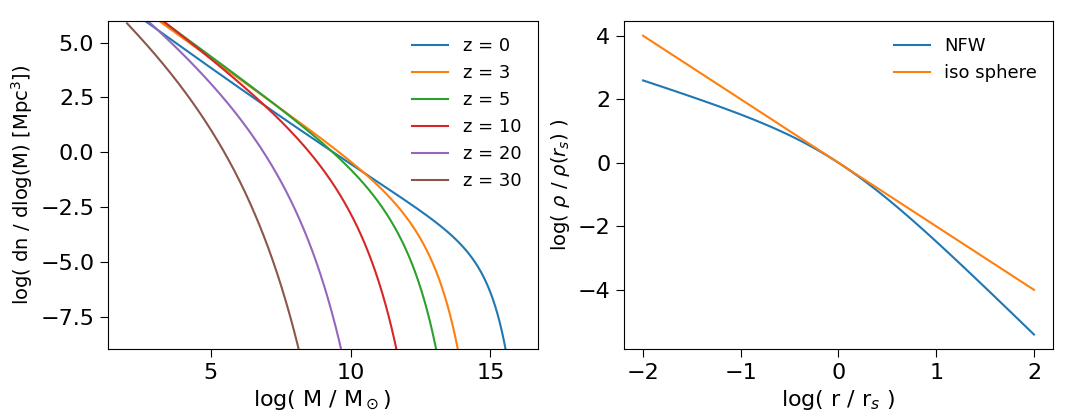
\includegraphics[width=1.0\textwidth]{plots/cosmo_3.png}
	\caption{\textit{Left}: halo mass function (number density of halos in a given mass logarithmic bin) for different redshifts $z$, according to the Press \& Schechter formalism (eq. \ref{eq:press_schechter}). The hierarchical growth of halos can be inferred from this plot, as low-mass halos are more abundant for high redshift, while higher mass halos are formed only at later redshifts. \textit{Right}: comparison between the isothermal sphere (eq.\ref{eq:iso_sphere}) and the NFW profile (eq. \ref{eq:nfw_profile}) for a dark matter halo. Radii are plotted in units of the scale radius $r_s$, while densities are divided by the density at scale radius $\rho(r_s)$. 
	}
	\label{fig:press_schechter_NFW}
    \end{figure}

\section{The first galaxies in the universe} \label{sec:birth_galaxies}


 In the basic picture we have portrayed in the last section, dark matter particles start to clump early in the primordial universe, and this process culminates with the formation of the first halos around redshift $z\sim30$. The resulting matter distribution, known as the \textit{cosmic web} because of its clumped and filamentary structure, has been confirmed by several large N-body simulations \citep[e.g.,][]{Springel:2005nw}. 
 
 However, so far we have completely ignored the fate of baryons: this is a key piece of the puzzle, as most of the information we can obtain about the universe is in the form of electromagnetic signals. Since dark matter does not interact with light, there is little hope to probe its structure and the general evolution of the universe if we do not understand how baryons evolve after they recombine and decouple from photons at last scattering. Unfortunately, these interactions with light and with themselves make baryons' behavior extremely difficult to model: unlike dark matter particles, baryons can combine in many atomic and molecular species, they can aggregate in complex structures, and cool or heat by emitting or absorbing light. 
 
 For these reasons, any predictions on their evolution involve a large number of physical processes, intertwined on a multi-scale level. In this section, we sketch the evolution of baryons as they fall into dark matter halos and form the first stars and galaxies. As these objects are created, they deeply impact the environment they are surrounded by, causing a profound modification of the global properties of the universe and finally making it similar to the one we observe today.
 
 \subsection{Jeans analysis} \label{sec:jeans}
 
 We have already introduced a (non-relativistic) description of the hydrodynamical properties of matter: mass conservation (eq. \ref{eq:mass_cons}), Euler (eq. \ref{eq:euler}) and Poisson (eq. \ref{eq:poisson}) equations are valid both for baryons and for dark matter. In the case of baryons, however, we cannot neglect the pressure term, and thus we need to relate the pressure to the density of the fluid by providing a thermodynamical closure.
 
 The most reasonable choice of closure is the adiabatic one: we assume the entropy is conserved, and thus the variations in pressure are proportional to the ones in density; the proportionality constant is the sound speed of the fluid:
 \begin{align}
   c_s^2 = \frac{\delta P}{\delta \rho} 
 \end{align}
 With this definition, we can rewrite the linear expansion of hydrodynamical equations (eqs. \ref{eq:euler_linearized1}--\ref{eq:euler_linearized3}) as:
 \begin{align}
    \Dot{\delta} &= - \frac{1}{a}\mathbf{\nabla}\times \mathbf{v}\\
    a(\Dot{\mathbf{v}}+H\mathbf{v}) &= -c_s^2\mathbf{\nabla}\delta  - \mathbf{\nabla}\delta\varphi\\
    \mathbf{\nabla}^2\delta\varphi &= 4\pi G\Bar{\rho}a^2(\delta+\delta_{dm}) 
 \end{align} 
 Note that in the Poisson equation, we have considered both the contributions from baryons and the ones from dark matter, as -- from the discussion in the last section -- dark matter perturbations are non-negligible. From this point onward, however, we will assume $\delta_{dm}=0$ and work with baryonic only perturbations: this simplistic assumption will allow us to determine some useful properties of baryons that will be important in later discussions.

 We can combine again the three hydrodynamical equations into a single one, obtaining the same result as eq. \ref{eq:euler_growing_delta} with a pressure contribution opposing the gravitational coupling:
  \begin{align}
    \Ddot{\delta} + 2H\Dot{\delta} = 4\pi G \Bar{\rho}\delta + \frac{c_s^2}{a^2} \mathbf{\nabla}^2 \delta 
 \end{align}
 The best way to deal with this kind equation is to work in the Fourier $\mathbf{k}$ domain; the Laplacian operator transforms into a $-\mathbf{k}^2$ factor, yielding:
 \begin{align}
    \Ddot{\delta}_\mathbf{k} + 2H\Dot{\delta}_\mathbf{k} + c_s^2\left( \frac{k^2}{a^2}-k_J^2\right)\delta_\mathbf{k},
    \label{eq:jeans}
 \end{align}
 where we have defined $k_J$ to be:
  \begin{align}
   k_J = \sqrt{\frac{4\pi G\Bar{\rho}}{c_s^2}}
 \end{align}
 Eq. \ref{eq:jeans} is a damped harmonic oscillator with a frequency $\omega^2=c_s^2\left( k^2/a^2-k_J^2\right)$: if the frequency is positive, the solutions are damped sines and cosines, and perturbations do not grow with time; a negative frequency, instead, corresponds to a growing solution that allows the perturbation to turn non-linear and ultimately leads to collapse (as we have already seen in the dark matter only case).
 Therefore, expressing the growth condition in terms of the \textit{Jeans scale} $\lambda_J$:
 \begin{align}
   \lambda_J = \frac{2\pi}{k_J} = \sqrt{\frac{4\pi c_s^2}{G\Bar{\rho}}}, \label{eq:jeans_scale}
 \end{align}
 we find that the overdensity at a (comoving) scale $\lambda$ collapses if the (physical) scale $a\lambda$ is greater than the Jeans scale $\lambda_J$. This condition can be well understood noting that $\lambda_J \sim c_s/\tau_{ff}$; $\tau_{ff}$ is the free-fall time, defined as:
 \begin{align}
\tau_{ff} = \frac{1}{\sqrt{G\rho}} \label{eq:free_fall}
 \end{align}
 Therefore, we are comparing the gravity timescale $\tau_{ff}$ with the time it takes pressure to act on the fluid ($a\lambda/c_s$): if the gravity timescale is short enough, information will not propagate fast enough for pressure to prevent the collapse of the structure. 
 
 We can turn the Jeans scale into a Jeans mass, in order to study which is the mass threshold for baryonic structures to collapse:
 \begin{align}
   M_J = \frac{4\pi}{3} \left(\frac{\lambda_J}{2}\right)^3\Bar{\rho} = \frac{4\pi^{5/2}}{3G^{1/2}}\Bar{\rho}_0^{-1/2}\,(c_s^2a)^{3/2},
 \end{align}
 where we have used the background density scaling $\Bar{\rho} = \Bar{\rho}_0 \,a^{-3}$. Thus, the Jeans mass evolves as the universe ages, allowing structures at different scales to collapse. In order to study this evolution, we have to determine the sound speed of baryons $c_s$. If baryons are decoupled from photons (after recombination), they can be considered as an ideal gas: thus, the adiabatic sound speed can be determined knowing that $P\rho^{-\gamma}\sim \mathrm{const.}$, with $\gamma$ being the adiabatic index ($\gamma=5/3$ for a monoatomic gas). Using the state equation for ideal gases, as well as the definition of mean molecaular weight $\mu$:
 \begin{align}
   P = nk_BT= \frac{\rho}{\mu m_p}k_B T, \label{eq:state_equation}
 \end{align}
 we find the following expression for $c_s$:
 \begin{align}
   c_s^2 =\gamma \frac{k_B}{\mu m_p} T,
 \end{align}
 The temperature of baryons, however, is not easy to determine. If baryons are moving freely along with the Hubble flow, their temperature scales as $T\propto a^{-2}$. This can be easily understood considering that $v \sim a^{-1}$, and that $k_B T \sim mv^2$. However, even after recombination, baryons are not completely free from interactions with photons. This is because a small number of electrons (and protons) are not able to form atoms before the recombination reaction gets out of equilibrium: these residual free electrons remain strongly coupled to CMB photons thanks to the relatively high cross-section of Compton scattering. The energy electrons exchange with photons is then redistributed among other baryons: this process keeps the temperature of baryons locked to the one of CMB photons down to redshift $z_t \sim 100$ \citep{barkana2005probing}. For this reason, we have to distinguish between two regimes: for $z>z_t$, the temperature of baryons is the same as the temperature of photons as the resulting Jeans mass does not depend on redshift (since $c_s^2 a \sim \mathrm{const.}$):
 \begin{align}
   M_J \approx 1.35\times 10^5 \,\msun
 \end{align}
 For $z<z_t$, instead, baryons temperature evolves independently from CMB photons, and the resulting Jeans mass depends on redshift as: 
 \begin{align}
   M_J = 5.73\times 10^3 \left(\frac{1+z}{10}\right)^{3/2} \,\msun \label{eq:jeans_threshold}
 \end{align}
 This study of the Jeans mass threshold is useful to determine the general behavior of baryons whenever gravitational collapse is involved. However, we have to keep in mind that we are completely neglecting the presence of dark matter: as dark matter halos form, their gravitational influence on baryons perturbations cannot be neglected, particularly at small scales. Therefore, in the next section, we will describe a different approach that can be used to study how baryons fall into the halos gravitational wells and form structures therein.
 

 \subsection{Baryons infall and cooling} \label{sec:infall_and_cooling}
  
  In order to study the evolution of baryons in the presence of dark matter beyond linear perturbation theory, we assume that halos have already formed, and examine how baryons can accrete into the potential wells $\varphi$ of these halos. Baryons will be attracted into these wells and will start concentrating in the inner regions of the halo until the pressure becomes high enough to counter the action of the gravitational potential $\varphi$. Ultimately, hydrostatic equilibrium can be reached:
  \begin{align}
   \mathbf{\nabla} P = -\rho \mathbf{\nabla} \varphi   
 \end{align}
  If we neglect every heat loss, then the process is adiabatic and we can relate density and pressure as $P\rho^{-\gamma}$ is conserved during the infall. The equilibrium quantities will be related to the background ones ($\Bar{P}, \Bar{\rho}$): 
  \begin{align}
   \mathbf{\nabla} \left(\frac{\rho}{\Bar{\rho}}\right)^\gamma = -\frac{\rho}{\Bar{P}} \mathbf{\nabla} \varphi = -\frac{\rho}{\Bar{\rho}} \frac{\mu m_p}{\Bar{T}} \mathbf{\nabla} \varphi,  
 \end{align}
 where we have used the state equation $\Bar{P}= (\Bar{\rho}/\mu m_p) k_B \Bar{T}$. The solution of this differential equation (with the background values as boundary conditions at infinity) is:
 \begin{align}
   \rho = \Bar{\rho} \left(1-\frac{2}{5}\frac{\mu m_p}{k_B \Bar{T}}\varphi\right)^{3/2} = \Bar{\rho} \left(1+\frac{4}{5}\frac{T_{vir}}{\Bar{T}}\right)^{3/2} \label{eq:baryon_accretion}
 \end{align}
 Note that the definition of the virial temperature $T_{vir}=-\mu m_p \varphi / 2 k_B$ is only approximately compatible with expression \ref{eq:virial_temperature}, as the relation between $\phi$ and the circular velocity $v_c$ depends on the specific shape of the halo density profile.
 
 In analogy with dark matter collapse, we can set a threshold value $\delta = \rho/\Bar{\rho} -1 > \Delta_c$ for baryons overdensities to be considered as collapsed structures. We choose $\Delta_c =100$: in this way, we can find the minimum virial temperature of a halo for it to accrete a relevant amount of baryons in its core. Eq. \ref{eq:baryon_accretion} gives the condition $T_{vir} \gtrsim 25 \Bar{T}$. We already determined the evolution of the baryons temperature for $z<z_t$, finding the scaling $T\sim a^{-2}\sim (1+z)^2$. We can also write the virial temperature in terms of the virial mass (eq. \ref{eq:virial_temperature}), in order to obtain a condition on the halo masses. We find:
  \begin{align}
    M > 8\times10^3 \left(\frac{1+z}{10}\right)^{3/2}\,\msun 
  \end{align}
 Therefore, we obtain that baryons accrete on halos with masses larger than a threshold which scales with redshift as $(1+z)^{3/2}$. Note that this result is quantitatively similar to the one we have obtained using Jeans analysis (eq. \ref{eq:jeans_threshold}): therefore, we can express this condition as $M>M_J(z)$. Of course, both approaches found on very coarse -- although different -- approximations, but they are aligned in suggesting a value of the mass scale for which baryons are actually able to clump and subsequently form complex structures. As halos formation proceed hierarchically (sec. \ref{sec:halos}), the presence of such a threshold suggests that baryons will start clumping in structures with $M\sim M_J(z)$, as soon as these halos are numerous in the universe. 
 
 As (quasi-)hydrodynamical equilibrium is reached, baryons form a self-gravitating structure where pressure prevents further collapse within the halo. The baryons' temperature at this point is comparable to $T_{vir}$, as the gas gets gravitationally heated during the infall. However, this state of equilibrium can be easily disrupted as baryons, unlike dark matter, can radiate away thermal energy: this key process explains how smaller structures such as stars and black holes form within the halo. The loss of energy, in fact, results in a loss of pressure support, and thus the gas has to contract to higher densities for it to be effective again.
 
 The \textit{radiative cooling} processes mentioned here will play a major role in the next chapters and will be thoroughly analyzed in chapter \ref{chap:model}. In this discussion, we just note how the efficiency of cooling (in the low-density regime) depends both on the gas temperature and on its composition. As primordial gas contains a negligible amount of metals (i.e., elements heavier than helium), cooling can only happen through lines excitation of hydrogen and helium. This poses a problem, however, as these cooling channels are not effective below $T\sim10^4\,\mathrm{K}$. This temperature corresponds to a virial mass of $M_{vir}\sim 10^8\,\msun$ at $z=10$: this would set a very high threshold for fragmentation to happen within the halo, and subsequently, delay star formation until lower redshifts. It turns out, though, that another cooling channel can open up at a temperature of $T\sim 10^3\,\mathrm{K}$ due to the rotational-vibrational transitions of $\mathrm{H}_2$ molecules. This channel sets a lower threshold for baryons' temperature to result in sufficient cooling. However, $\mathrm{H}_2$ is not always present: even a small amount of UV radiation in the \textit{Lyman-Werner (LW) band} ($10.2-13.6\,\mathrm{eV}$) can dissociate the molecule in a two-step photo-dissociation mechanism known as \textit{Solomon process} \citep{draine_bertoldi} (see also \ref{sec:radiation_fields}).
 
 For this reason, baryons' collapse in the inner regions of dark matter halos is usually described as a two-fold process: first, baryons cool down via molecular transitions in halos with a virial mass around $M_{vir}\sim10^6\,\msun$ (known as \textit{minihalos}). As the first stars form and emit UV radiation (see next section), $\mathrm{H}_2$ stops playing a major role as a coolant and galaxy formation is delayed until baryons in more massive halos ($T_{vir}\sim10^4\,\mathrm{K}$ and $M_{vir}\sim 10^8\,\msun$) emit $\mathrm{Ly}\alpha$ radiation via collisional excitation of hydrogen atoms.
 

 
 \subsection{First light and reionization} \label{sec:first_lights_reionization}
 
 Once the gas cools and loses pressure support, it collapses in the inner regions of the halo until it is supported by its angular momentum. The resulting self-gravitating structure resembles a rotating disk: a protogalaxy has formed. At this point, the gas tends to become self-gravitating (i.e., dominated by its own gravity rather than that of the dark matter). Even though the gravitational influence of the halo is still important to determine the global evolution of the galaxy, its role becomes secondary on a local level. Therefore, Jeans analysis (sec. \ref{sec:jeans}) can be applied to study further collapse and fragmentation of gas. 
 
 Fragmentation occurs at scales comparable with the Jeans scale $\lambda_J$ (eq. \ref{eq:jeans_scale}). If the cooling timescale is smaller than the dynamical one (i.e, the free-fall time $\tau_{ff}$) then the gas evolution can be considered isothermal because the energy loss is primarily compensated by an increase in density. For a constant temperature, however, the Jeans mass scales as $\rho^{-1/2}$: for this reason, as the density increases, the Jeans mass decreases, and the gas breaks up into even smaller clumps. This process leads to the formation of \textit{Giant Molecular Clouds} (GMCs). GMCs can have very different properties, as they ultimately arise from the complex interplay of cooling, gravity, turbulence, and magnetic effects: their density ranges from $10^2\,\mathrm{cm}^{-3}$ in the external regions to $10^7\,\mathrm{cm}^{-3}$ in the densest cores. In these cores, gas can ultimately collapse and reach the extreme densities necessary to ignite nuclear fusion, forming the first protostars. Note, however, that the mechanism in which stars are formed is extremely difficult to model, and many of its details are still poorly understood.
 
 %in galaxy formation models, star formation is usually implemented using some kind of prescription on the physical conditions gas has to reach in order to form a star, as well as on the efficiency of this formation process. 
 
 The birth of the first stars in the universe marks a key passage in its evolution: it is the end of the \textit{Dark Ages}. From the epoch of recombination, in fact, the universe is filled with neutral gas with a primordial composition (i.e., hydrogen, helium, and traces of metals). The properties of this gas are quite uninteresting from an astrophysical perspective: aside from the H (and $^3$He) hyperfine transition line, no electromagnetic radiation is emitted by this neutral gas. Therefore, the growth of perturbations, the formation of dark matter halos, and the collapse of baryons happen in an overall dark universe. As the first stars shine, everything changes: photons travel again in the universe, interacting with the neutral hydrogen, and, in principle, reaching our telescopes -- although we still lack the technical capabilities to observe the light emitted from first stars \citep{rydberg2013detection}. 
 
 The interaction between photons emitted by the first stars -- known as \textit{PopIII stars} -- and hydrogen atoms has a huge impact on the properties of the entire universe: photons are able to ionize the Inter-Galactic Medium (IGM), i.e., the reservoir of neutral gas that does not belong to collapsed structures and fills the universe since recombination.
 In order to appreciate the relevance of this process, we can consider the efficiency of hydrogen nuclear fusion. The energy liberated per hydrogen atom is approximately:
 \begin{align}
   E = 0.7\% \,m_p c^2 \approx 6\times 10^6\,\mathrm{eV}
 \end{align}
 As it takes only $13.6 \,\mathrm{eV}$ to ionize an hydrogen atom, it suffices to convert into stars a small fraction (around $10^{-5}$) of neutral gas to ionize it all. This process is known as \textit{reionization}, and it represents the last phase transition that the universe undergoes in its history. Current models place the Epoch of Reionization (i.e., the time at which the universe is fully ionized) around $z\sim6-7$ \citep{mesinger_2016}.
 
 Reionization is a complex process, as it is directly influenced by the physics of structure formation on a multi-scale level: ionization fronts travel from single stars to intergalactic distances. We can sketch the process using a simple analytical model as follows: we consider a single, star-forming galaxy surrounded by a neutral IGM. As ionizing photons are emitted by the galaxy, they travel freely until they find the boundary between the neutral and ionized gas: ultimately, they are able to drive an ionization front that travels further into the IGM. The size $R_i$ of the resulting \HII (i.e., ionized hydrogen) region changes according to the following relation:
 \begin{align}
   \langle n_\mathrm{H}\rangle 4\pi R_i^2 \frac{\d R_i}{\d t} = \dot{N}_\gamma- \alpha \langle n_\mathrm{H}^2\rangle \frac{4\pi}{3} R_i^3
  \end{align}
  In this formula, the velocity of the ionizing front depends on the total rate of ionizing photons emitted by the central galaxy $\dot{N}_\gamma$, as well as on the rate of hydrogen recombination (which causes the ionization fraction to decrease and thus slows down the shell growth). The former term can be written as:
  \begin{align}
  \dot{N}_\gamma = \frac{\d}{\d t}\left(\fesc\, N_b\, f_*\, N_{\gamma,b}\right) \approx  \fesc \, f_*\, N_{\gamma,b}\,\frac{\d N_b}{\d t}
  \end{align}
  Here, $\fesc$ is the \textit{escape fraction} (i.e., the fraction of ionizing photons that are able to escape from the galaxy), $N_b \,f_*$ is the total number of baryons in stars, and $N_{\gamma,b}$ is the rate of photons emitted by a single stellar baryon. The second equality follows if we assume that only the total number of baryons inside the galaxy $N_b$ changes significantly over time: this approximation neglects the changes in the properties of stellar population, feedback, and galaxy's morphology, and thus, it is valid only for a very coarse model. Introducing also the clumping factor $C= \langle n_\mathrm{H}^2\rangle/  \langle n_\mathrm{H}\rangle^2  $, we can rewrite the equation describing the evolution of the ionized volume $V_i$ as:
  \begin{align}
   \dot{V}_i = \langle n_\mathrm{H}\rangle^{-1} \,\fesc \, f_*\, N_{\gamma,b}\,\dot{N}_b - \alpha C \langle n_\mathrm{H}\rangle\,V_i \label{eq:volume_reionization}
  \end{align}
  Considering the global picture, at the Epoch of Reionization the universe will be filled by these expanding ionized regions that eventually overlap and merge creating larger \HII structures until the whole IGM becomes ionized. We can compute the filling factor of \HII regions, $Q_i$, by summing over many ionized volumes and dividing by the total volume of the universe $Q_i = \sum_i V_i / V_\mathrm{tot}$. The equation governing the evolution of $Q_i$ follows directly from eq. \ref{eq:volume_reionization}:
   \begin{align}
   \frac{\d Q_i}{\d t} = \fesc \, f_*\, N_{\gamma,b}\,\frac{\d f(>M_\mathrm{min},z)}{\d t} - \alpha C \langle n_\mathrm{H}\rangle\,Q_i, \label{eq:reionization_equation}
  \end{align}
  where we have rewritten the fraction of baryons collapsed in galaxies, $\sum_i N_{b,i}/(\langle n_\mathrm{H}\rangle\,V_\mathrm{tot})$, using the collapsed fraction of dark matter particles (eq. \ref{eq:collapsed_fraction}) in halos with masses larger than a threshold value $M_\mathrm{min}$ (see discussion in section \ref{sec:infall_and_cooling} for more details). 
  
  The picture here presented describes the main features of reionization in a very sketchy way. A more detailed treatment is possible using numerical/statistical techniques \citep[e.g.,][]{mesinger_2016}. However, these simple arguments are useful as they allow us to determine the key parameters that steer the evolution of $Q_i$. $f_*$ and $N_{\gamma, b}$ are connected with star formation, as they describe the efficiency of SF and the properties of stellar radiation respectively; we will deal with these parameters in section \ref{sec:star_formation}. 
  
  The two other arbitrary parameters we have introduced are the escape fraction $\fesc$ and the clumping factor $C$. These are particularly important as, depending on the detailed internal structures of the first galaxies and on their surroundings, they are largely unconstrained by observations. In particular, the escape fraction directly depends on the morphology and the distribution of column densities in the inner regions of galaxies, as ionizing photons are mainly absorbed by the neutral and dusty ISM. Both observations in the FUV band and numerical simulations (see below) are used to pinpoint the value of $\fesc$. 
  However, no consensus has been reached yet, as even the order of magnitude of $\fesc$ and its trends with mass, luminosity, and redshift are still to be established. A number of different works have tried to infer $\fesc$ from observations, obtaining values ranging between $\fesc \approx 1\,\%$ and $\fesc \approx 20\,\%$ \citep[e.g.,][]{inoue2006escape}. However, these numbers depend on a few underlying assumptions (e.g., star formation history, IGM absorption along the line of sight, absence of spurious contamination) that are difficult to benchmark. Simulations find values of $\fesc$ that tend to decrease with mass - as a consequence of a denser and more clumped ISM - and to increase with redshift. Reported values are $\fesc \approx 0.15- 0.6$ for $M_{vir}\lesssim 10^{6-7}\,\msun$, $\fesc \approx 0.05 -0.4$ for $M_{vir}\lesssim 10^{8-9}\,\msun$, $\fesc\approx 0.01- 0.07$ for $M_{vir}\sim 10^{10-11}\,\msun$ \citep{xu2016galaxy,wise2014birth, ma2020no}. However, other authors find much lower values for $\fesc$, as low as $10^{-5}$ \citep{paardekooper2015first}.
  The discussion on the relevance of the escape fraction in determining the characteristics of reionization is particularly interesting in the context of our thesis work, as $\fesc$ will play an important role in our model (chapter \ref{chap:model}).
 
 
 
 

\section{Basic physics in galaxy evolution} \label{sec:physics_galaxies}
  


 In the last section, we have outlined the process of galaxy formation and its direct implications on the universe's evolution. Here, we face the problem of studying galaxies as they evolve with the universe. This is an extremely complex task, because galaxy evolution is led by the interplay of many different processes at different scales and levels. 
 
 There exist different techniques that have succeeded in describing how galaxies evolve with time, matching observable quantities such as luminosity functions (LFs), chemical compositions, and density distributions. Numerical simulations are the most explicit way to model the formation and evolution of galaxies in a subset of a virtual universe whose initial conditions are set to match real observations. The basic idea is to solve numerically the equations for gravity, hydrodynamics, thermodynamics, and chemistry, using particles and/or grid cells that represent dark matter, gas, and stars. Even though their resolution and their spatial extension are limited by computational exigencies, these simulations can capture the intrinsic complexity of a variety of different physical processes. Small-scale processes (e.g., star formation) are implemented using effective prescription and parameters that are fine-tuned to match observations. A few years ago, many different simulations have finally succeeded in reproducing galaxies that are statistically compatible with the ones we observe in the local universe (see Figure \ref{fig:eagle}). 
 
 A different approach one can take in order to follow galaxies' evolution is represented by "\textit{Semi-Analytic Models}" (SAMs).  This method focuses on a set of simplified equations that describe the mutual interactions between different components (e.g., inflowing gas, outflowing gas, stars, cool ISM) via some parameters that are tuned according to observations (just as numerical simulations). The growth of halos and galaxies is followed using a \textit{merger tree}, i.e., treated in a statistical way adopting a prescription such as the Press-Schechter (eq. \ref{eq:press_schechter}).

 In the next few paragraphs, we give rudimentary physical insights into the main factors that are thought to dominate the galactic evolution process: cosmological gas accretion, star formation, and feedback processes. These are included both in SAMS and in cosmological simulations, and concur to determine how a galaxy grows with time, forming new stars and increasing its size and mass content, as well as changing its global observable properties. 
 
 
\begin{figure}
	\centering
	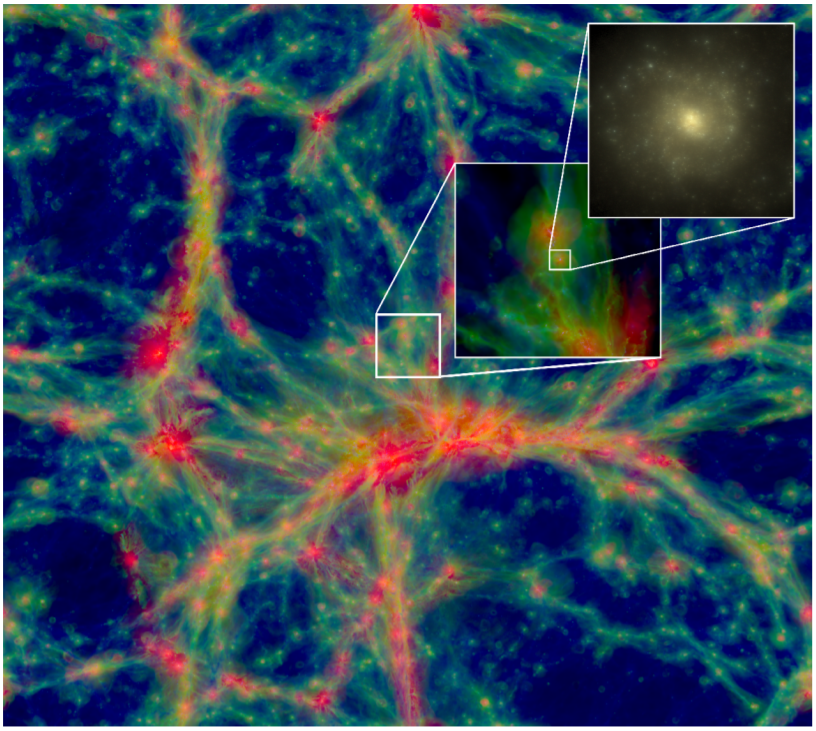
\includegraphics[width=0.57\textwidth]{plots/eagle.PNG}
	\caption{A snapshot of 100 × 100 × 20 cMpc (comoving-Mpc) taken from the EAGLE cosmological simulation \citep{schaye2015} at $z=0$. The intensity represents the gas density, while the color codes the gas temperatures from cool gas (blue) to the hotter one (red). The insets zoom on a region where a MW-like galaxy resides. 
	}
	\label{fig:eagle}
    \end{figure}
    
    
  \subsection{Gas accretion} \label{sec:accretion}
  
  Gas accretion is important to determine the evolution of the galaxy because, as stars form, they consume the cold gas reservoir inside the galaxy. Accretion from the IGM renovates this reservoir by providing new gas that can fuel the process of star formation. Therefore, the rate at which the gas accretes to the galaxy directly affects its gaseous and stellar content. 
  
  We have already described how baryons are attracted into the potential wells of dark matter halo, and form a quasi-hydrostatic hot gaseous halo that starts to cool down radiatively if the virial temperature is above a certain threshold (section \ref{sec:infall_and_cooling}). This process is responsible for galaxy formation, but it continues to provide new cold gas to the galaxy along the entire evolution process. 
  
  We can refine our discussion on gas accretion and cooling by introducing the gas cooling time $\tau_\Lambda$:
  \begin{align}
   \tau_\Lambda(r) = \frac{E_{in}}{n\,\Lambda(T)} = \frac{1}{\gamma - 1}\frac{\mu m_p k_B T}{\rho(r)\Lambda^\mathrm{(cool)}(T)} \label{eq:tcool}
  \end{align}
  $E_{in}= k_B T/(\gamma-1)$ is the internal energy of the gas, while $\Lambda^\mathrm{(cool)}(T)$ is the cooling rate (measured in $[\mathrm{erg}\,\mathrm{cm}^3\,\mathrm{s}^{-1}]$). These quantities will be explored in details in chapters \ref{chap:outflows}--\ref{chap:model}, as they constitute the building blocks of the model presented by this work. 
  
  Comparing the cooling time $\tau_\Lambda$ with the free-fall time $\tau_{ff}$ (eq. \ref{eq:free_fall}), we find a cooling radius $r_{cool}$ for which $\tau_\Lambda(r_{cool})=\tau_{ff}(r_{cool})$. Given the density dependency of these two time scalings, in the region inside $r_{cool}$ the gas cools effectively -- as its cooling time is shorter than the free-fall one --, while in the outer region dynamical effects prevail over cooling -- as the free-fall time gets shorter. Provided that a hot gaseous halo has formed as described in sec. \ref{sec:infall_and_cooling}, the gas will start cooling for $r<r_{cool}$. Therefore, we can write the accretion rate $\Dot{M}_{acc}$ as:
  \begin{align}
   \dot{M}_{acc} \sim 4\pi \rho(r_{cool})\frac{\d r_{cool}}{\d t}
  \end{align}
  In this picture, the gas is slowly accreted from the hot halo reservoir as the cooling threshold moves outside from the center. This is commonly known as "hot accretion mode".
  
  However, if the cooling radius is greater than the virial radius $r_{vir}$, then cooling is always efficient: no halo formation takes place, as the gas can cool efficiently and fall directly in the inner regions of the halo. The accretion rate, in this latter case, is only bounded by the dynamical timescale: for this reason, it is common to model this process assuming that the gas can flow into the halo on a free-fall time. The gas mass, in turn, depends on the halo mass, as the gas is accreted along with dark matter. These "cold modes" of accretion are much more efficient at providing cold, ready-to-use gas to the galaxy. For this reason, they are thought to play a major role in governing the cold gas mass budget of the galaxy, particularly at higher redshifts. As cosmological hydrodynamical simulations have shown, these modes occur along dense and cold filaments \citep{kerevs2005galaxies}, reflecting the filamentary structure of the dark matter "cosmic web" (e.g., see figure \ref{fig:eagle}). 

  As a final note, we point out that accretion is not the only way in which galaxies increase their gas reservoir. Along with their dark matter halo host, in fact, galaxies can merge and form more massive systems, in a hierarchical process that leads to galaxy growth with cosmic time. Mergers happen as a result of close encounters between different structures, and thus are more frequent as the density of objects increases. For this reason, they are thought to play an important role in driving galaxy mass growth at higher redshifts, as well as in galaxy groups and clusters. Besides increasing galaxy masses and providing new gas reservoirs, mergers are also important because they can trigger star formation as they create shocks in the gas that locally increase its density \citep{conselice_mergers}. 

  \subsection{Star formation and its consequences} \label{sec:star_formation}

  As described in section \ref{sec:first_lights_reionization}, the first stars in the universe formed out of the coldest and densest regions in Giant Molecular Clouds. These first structures -- named \textit{PopIII stars} -- are thought to have very different properties compared to the stars we observe in the local universe: they are more massive, more luminous, hotter, and metal-free \citep{haemmerle2020formation}. 
  
  These properties have important consequences: first of all, massive and luminous stars have a higher effective temperature. For this reason, the spectrum of these stars contains a larger fraction of ionizing photons (with energies greater than $13.6\,\mathrm{eV}$) as well as a greater number of photons in the LW band ($10.2-13.6\,\mathrm{eV}$). We have already discussed (sec. \ref{sec:infall_and_cooling}--\ref{sec:first_lights_reionization}) how these photons impact the galactic environment and the universe as a whole: they start the process of cosmic Reionization by creating ionizing bubbles in their surrounding medium, and they photo-dissociate $\mathrm{H}_2$ molecules hampering gas cooling in lower mass halos. Ultimately, radiation from these stars contributes to forming a background of UV photons that affects the properties of the Inter- and Circum-Galactic Media (IGM/CGM) by photo-heating and photo-ionizing the gas. The UV background (UVB) will play a critical role in our model, and we will study in detail its effects in section \ref{sec:radiation_fields}. 
  
  Another important characteristic of PopIII stars is their brief lifetime. Since the available energy for nuclear fusion is proportional to the stellar mass $M$, the stellar lifetime $\tau_s$ scales as:
  \begin{align}
      \tau_s \sim \frac{Mc^2}{L} \sim M^{-5/2},
  \end{align}
  where we have used the mass-luminosity relation $L\sim M^{7/2}$ for massive stars \citep{griffiths88}. Thus, massive stars consume their energy reserve faster and they soon run out of fuel. For a star of about $\sim 10\,\msun$, this lifetime is around tens of Myrs: this is much shorter than the dynamical timescale of the galaxy. For this reason, as the galaxy evolves dynamically, many stars form and die. The death of a massive star culminates with the collapse of the star's core: this results in a catastrophic explosion followed by shock waves propagating into the surrounding gas \citep{ostriker_supernovae} -- this phenomenon is known as Supernova (SN). Energy is injected in the Inter-Stellar Medium (ISM) by the interaction of the expanding shell with the surrounding gas. The amount of energy a single supernova can liberate is astounding: in low-mass halos, it can be greater than the gravitational binding energy of the gas. For this reason, supernovae events exert a profound influence on the life of the host halo: they can launch powerful outflows that drive gas out into the IGM, competing with the gas accretion process in determining the ISM mass budget. 
  
  Moreover, the core-collapse of a massive star often results in the formation of a remnant object, that can be either a \textit{neutron star} or a \textit{black hole}. Black holes forming out of the first stars are particularly interesting, as they are one of the candidates to be the seeds of the Super-Massive Black Holes (SMBHs) we observe today in virtually any galaxy with a central bulge \citep{Latif:2016qau}. Along with stars, SMBHs are considered to be the primary cause for driving galaxies growth: a tight correlation is in fact found between the properties of SMBHs and the ones of the galactic inner regions, strongly suggesting an interconnected coevolution process \citep{Kormendy:2013dxa}. The most straightforward way in which SMBHs couple with their host galaxies is through the energy released in their active phase of accretion: as gas falls within the black holes' potential well, it is heated to extremely high temperatures and it radiates away a considerable fraction of its binding energy. The efficiency of this process is extremely high: on average, it is an order of magnitude greater than the efficiency of Hydrogen nuclear fusion. SMBHs in their active phase are known as \textit{Active Galactic Nuclei} (AGN) -- or equivalently as \textit{Quasars} (QSOs).    
  
  Finally, the death of a massive star has another important consequence: the external layers of the star are ejected out and they mix with the cold ISM. In this way, the gas is enriched with the metal elements formed inside the star thanks to nuclear fusion. Gas exchange between galaxies and their surroundings is then responsible for bringing metals into the IGM, ultimately polluting the primordial gas everywhere in the universe (chapters \ref{chap:results}--\ref{chap:conclusion}). The process of metal enrichment has a dramatic impact on subsequent stellar evolution, as it marks the end of metal-free (PopIII) star formation. Metals such as carbon and oxygen, in fact, allow the gas to cool well below the hydrogen threshold of $10^4\,\mathrm{K}$ (section \ref{sec:cooling}): lower temperatures result in stronger fragmentation and clumping, ultimately leading to a new generation of \textit{PopII stars} characterized by lower masses and higher metallicities (i.e., mass fraction of metals in the gas). Studies show that the transition between PopIII and PopII stars happens when a metallicity threshold $Z_{crit}\sim 10^{-3.5}-10^{-5}$ is reached \citep{bromm2001fragmentation}. This value is relatively low, as in $M_{vir}\sim10^8\,\msun$ halos, it can be attained thanks to the metal yields of a few SNe explosions \citep{karlsson2008uncovering}.
  
  Globally, star formation depends on the availability of cold gas in the ISM. A possible parametrization for the star formation rate (SFR) in a galaxy is:
  \begin{align}
    \mathrm{SFR}(t) = \dot{M}_\mathrm{star} = f_* \,\dot{M}_{acc}(t) \label{eq:feedback_parameter}
  \end{align}
  The parameter $f_*$ expresses the role of \textit{feedback mechanisms} acting on the gas: these are the subject of the next section.
  Note that, in this relation, we have assumed that the gas contributes to forming stars as soon as it is accreted in the ISM. We should caution that this assumption is not true in general: the exact link between accretion and star formation is still to be established, as both observations and theoretical arguments struggle to explain this connection in detail \citep[e.g.,][]{almeida2016}. This problem can be mitigated by considering more sophisticated prescriptions for star formation (e.g., defining a time distribution for the probability of forming stars after accretion). 
  
  Once a star formation rate history $\mathrm{SFR}(t)$ has been established, one can describe the evolution of a stellar population in a galaxy by assuming an Initial Mass Function (IMF) (i.e., the initial probability of forming a star of mass $m$). Common choices for PopII stars IMFs include (broken) power laws of the form $\Phi(m) \propto m^{-\alpha}$ (e.g., $\alpha = -2.35$ for the Salpeter IMF \citep{salpeter1955}). Knowing the spectral emission for a single star $f_\mathrm{star}(t,Z)$ as a function of time $t$ and metallicity $Z$, then, it is possible to sum the light emitted from all the stellar sources at a time $t$ to come up with a prediction for the spectral emission of a galaxy. This can then be compared to observations in order to assess the validity of the assumptions made in the model; this approach is known as \textit{Stellar Population Synthesis} (SPS). The final spectrum at a given time $t$, $f_\mathrm{CSP}(t)$, will read:
  \begin{align}
    f_\mathrm{CSP}(t) = \int_{0}^{t} \int_{0}^{Z_\mathrm{max}}\int_{m_\mathrm{min}}^{m_\mathrm{max}(t)} \mathrm{SFR}(t-t')\,P(Z; t-t')\,\Phi(M)\, f_\mathrm{star}(t',Z) \,e^{-\tau_d(t')}\,\d t'\,\d Z\,\d M \label{eq:galaxy_spectrum}
  \end{align}
  where $Z_\mathrm{max}$, $m_\mathrm{min/max}$ are the extremal values for the metallicity and the stellar masses respectively, and $P(Z;t)$ is the time-dependent metallicity distribution. The negative exponential term accounts for dust attenuation: $\tau_d$ is the averaged dust optical depth in the galaxy, obtained integrating the dust absorption coefficient $\alpha_d$ along different line of sights (LOS).
  
  \begin{figure}
	\centering
	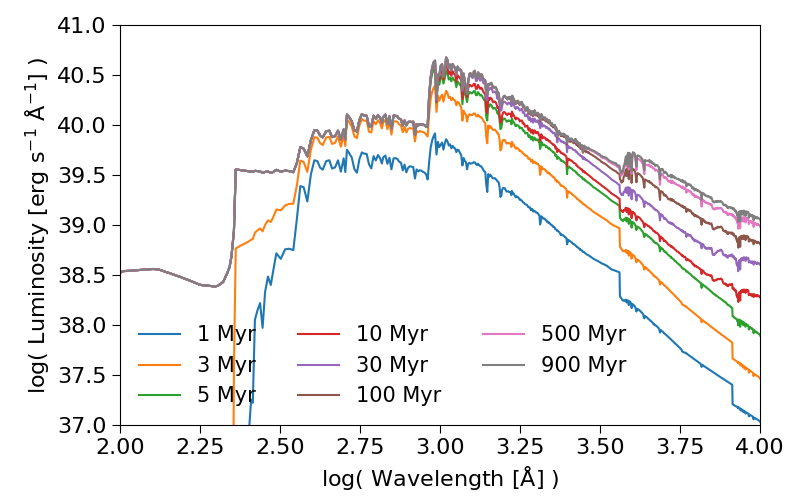
\includegraphics[width=0.6\textwidth]{plots/starburst99.PNG}
	\caption{Luminosity of a galaxy as a function of the wavelength, created using the Stellar Population Synthesis code \code{starburst99} \citep{leitherer1999}. The different curves refer to different galactic evolutionary times (between $1\,\mathrm{Myr}$ and $1\,\mathrm{Gyr}$). The galaxy has a SFR $=1\,\msun$, a metallicity $Z=0.040$; the IMF is taken to be Salpeter-like with a lower mass threshold of $1\,\msun$ and a higher mass threshold of $100\,\msun$.
	}
	\label{fig:scp}
    \end{figure}
    
  Figure \ref{fig:scp} represents an instance of these spectra for different time snapshots, created using the SPS code \code{starburst99} \citep{leitherer1999}. These spectra are generally peaked in the UV - where the light from the youngest and brightest stars is concentrated - and they decrease in intensity as the wavelength increases. However, this general behavior does not include the contribution of dust. In fact, dust absorbs radiation and thus heats up to hundreds of Kelvin, emitting thermal radiation in the IR. In order to account for this radiation, a second term has to be added inside the integral in eq. \ref{eq:galaxy_spectrum}.
  

  \subsection{Feedback and the baryon cycle} \label{sec:feedback}
  
  
  We have already examined how the birth of PopIII stars influences the environment in which they live. These are all instances of feedback mechanisms: the term feedback refers to the fact that the birth of a star has a relevant impact on the subsequent rate (and properties) of star formation itself. In a broader sense, feedback is the expression of the complex interconnection between the components of a galaxy: hot and cold gas, stars, black holes, radiation, and dark matter. Generally, however, the term feedback is primarily used to describe the effect of winds driven by massive stars, Supernovae, and AGN on interstellar and intergalactic gas. These winds are able to suppress star formation by heating the cold gas and removing it from the galaxy, as well as by preventing the circumgalactic gas to fall into the galaxy and thus reducing the accretion rate; at the same time, they may have also a positive effect on star formation, as they produce shocks that can compress the gas and trigger the formation of stars \citep{silk2009global, ishibashi2012active}.
  
  We will devote the next chapter to the study of the origin, the effects, and the properties of galactic winds. Here, we examine these feedback mechanisms in the light of galactic evolution models. Appreciating the major role played by feedback in driving galaxy evolution has been one of the key steps in the last decades of research in the field. The success of numerical simulations in recreating the observed galaxies' population largely relies on a more accurate treatment of feedback prescriptions \citep{Vogelsberger:2019ynw}.
  
  
  Many observational hints point towards the fact that feedback cannot be neglected when describing how a galaxy forms new stars with time. The most convincing argument comes from the study of the galaxy mass function \citep{Kormendy:2013dxa} (i.e., the number density of galaxies having a certain stellar mass): according to a naive application of the $\Lambda\mathrm{CDM}$ model, this galaxy mass function should have the same shape of the halo mass function (sec. \ref{sec:halos}), as baryonic clumping is mainly driven by the dark matter distribution in the universe. However, there are strong evidences for suppression of the galaxy mass function both at the lower end and at the higher one of the mass spectrum (fig. \ref{fig:halo_stellar}). These discrepancies can be explained by the hindering action of feedback by SNe and AGN respectively.
  
  In order to understand why the effects of feedback cannot be neglected, we can compare the energy released by SNe and AGN activity to the gravitational energy that keeps the gas bound to the halo. Defining the total baryon mass $M_g$, this energy can be approximately written as:
  \begin{align}
   E_b = \frac{GM_h}{r_{vir}} M_g =  v_c^2 M_g,
   \end{align}
  If the energy injected in the gas is greater than this quantity, then outflows are able to evacuate baryons from the galaxy, extinguishing the cold gas reservoir and thus quenching star formation completely. 
  
  Supernovae inject an amount of energy in the ISM which can be written simply as the energy released by a single SN ($E_{0,\mathrm{SN}}$) multiplied by the total number of SNe $N_\mathrm{SN}$. In turn, this latter quantity depends on the frequency of SNe per unit mass $\nu_\mathrm{SN}$, and on the total stellar mass in the galaxy: integrating eq. \ref{eq:feedback_parameter}, this mass can be related to the baryon mass via the feedback parameter $f_*$. The energy injected by SNe in the surrounding medium heats the gas, making it buoyant and ultimately leading to the formation of a wind. We can relate the injected energy to the energy that effectively couples to outflows via an efficiency parameter $\varepsilon$, in order to account for the fraction of energy that is radiated away by the gas before it can drive winds out of the galaxy. Ultimately, the total energy due to SNe acting dynamically on the gas is: 
  \begin{align}
   E_\mathrm{SN} =  E_{0,\mathrm{SN}} \,N_\mathrm{SN} \, \varepsilon_\mathrm{SN} = E_{0,\mathrm{SN}}\,\nu_\mathrm{SN}\, f_*\,M_g\,\varepsilon_\mathrm{SN}
  \end{align}
  When this energy is greater than the binding energy of the gas, star formation is completely suppressed because of feedback. Therefore, there is a maximum value for the feedback efficiency $f_{*,\mathrm{max}}$ that cannot be exceeded, as a larger star formation rate ultimately leads to quenching via the action of SNe. Using eq. \ref{eq:circular_velocity} for the circular velocity, we obtain:
  \begin{align}
    f_{*,\mathrm{max}} = \frac{v_c^2}{E_{0,\mathrm{SN}}\,f_\mathrm{SN}\,\varepsilon_\mathrm{SN}} = \left(\frac{\varepsilon_\mathrm{SN}}{10^{-3}}\right)^{-1}\,\left(\frac{M_h}{10^8\,h^{-1}\msun}\right)^{2/3}\,\left(\frac{\Omega_m}{\Omega^z_m}\frac{\Delta_c}{18\pi^2}\right)^{1/3}\,\left(\frac{1+z}{10}\right)
  \end{align}
  This result implies that, even for a very small coupling constant $\varepsilon$ between SNe and galactic winds, star formation is effectively hampered by feedback. This mechanism can explain the suppression in the low mass range of the galaxy mass function (figure \ref{fig:halo_stellar}), as the resulting stellar mass scales with $M_* \sim f_* \,M_g \sim f_* \,M_h$, and at low masses the $f_*$ dependence on $M_h$ shatters the proportionality between the galaxy mass and the halo mass. 
  
  Note that this maximum efficiency sets a significant constraint to star formation only for low mass halos, because at high masses the binding energy is greater, and thus SNe activity cannot provide enough energy to the gas to free it from the gravitational influence of the halo. However, as halo masses increase, SMBHs come into play. We can repeat the same argument as before, comparing the baryons binding energy with the energy emitted by an AGN times an efficiency parameter $\varepsilon_\mathrm{BH}$. This time, however, energy made available by feedback is at least one order of magnitude greater, as the efficiency of AGN emission is a substantial fraction ($\sim 10^{-1}$) of the black hole mass, and this latter quantity scales with the galaxy mass roughly as $M_\mathrm{BH} \sim 10^{-3}\, M_*$ \citep{Kormendy:2013dxa}. Therefore, AGN can be effective at quenching galaxy growth even in far more massive galaxies. For this reason, the abrupt suppression observed in the high mass range ($M_*\sim 10^{11.5-12}\,\msun$) of the galaxy mass function (figure \ref{fig:halo_stellar}) is conventionally ascribed to the influence of AGN. This claim is now supported by both observational studies and simulations, which are shedding light on the mechanisms through which this kind of feedback acts and their consequences on galaxy evolution \citep{Harrison:2018jvh, Sijacki:2007rw, Hopkins18, Beckmann:2017luq}.
  
\begin{figure}
	\centering
	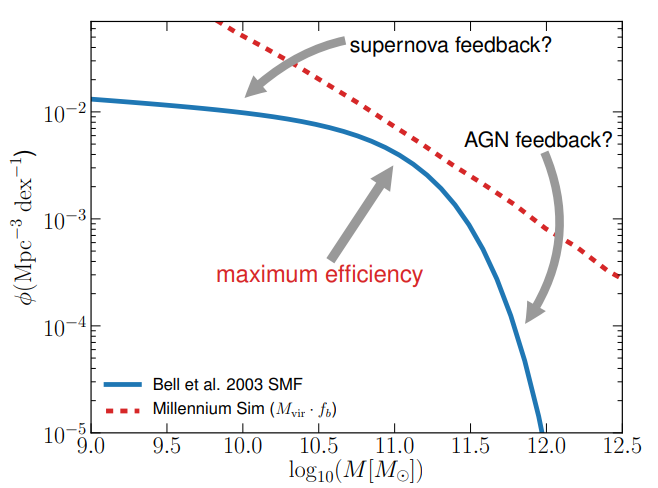
\includegraphics[width=0.58\textwidth]{plots/feedback.png}
	\caption{A comparison between the observed galactic stellar mass function (blue) and the distribution expected from the $\Lambda\mathrm{CDM}$ model for perfectly efficient star formation (red). The former is taken from \citet{bell2003optical}, while the latter is obtained by considering the HMF from the Millennium Simulation \citep{Springel:2005nw} and multiplying it for the universal baryon fraction.
    The different slopes at low and high masses between the two lines indicate that star formation is less efficient in these regions. Taken from Mutch et al. \citep{mutch2013simplest}.
	}
	\label{fig:halo_stellar}
    \end{figure}
  


 Besides impacting the star formation rates in galaxies, the presence of feedback in the form of outflowing gas has dramatic consequences for the nearby CGM/IGM. The Circum-Galactic Medium is conventionally defined as the region between the external limits of the galaxy and the virial radius of its dark matter halo. As gas flows out of the galaxy, it floods into the CGM, affecting its properties such as composition, temperature, density, and radial velocity. The wind interacts hydrodynamically with the pre-existing CGM, and gravitationally with the halo's dark matter. Ultimately, the fate of the outflowing baryons depends on both of these processes: they can either be shocked and slowed down, or they can expand freely into the IGM. In the first scenario, the gravitational pull of the DM halo stops the outflows completely, and baryons eventually fall back into the galaxy, creating a "\textit{galactic fountain}" \citep{oppenheimer2006} that refuels the ISM with the same recycled gas that had left the galaxy in the form of an outflow. In the second one, baryons can leave the galaxy and mix with the primordial gas that does not reside in any collapsed structure. This mixing process alters the composition of the primordial IGM, as its metallicity increases because of the contribution of outflowing gas. Metal enrichment (or pollution) of the IGM/CGM via galactic outflows is considered to be the most promising way to explain why roughly half of the metals in the local universe are located outside galaxies, even though they were formed only inside them \citep{menard2010measuring}.
 
 The evolution of outflows as they expand into the CGM parallels with the presence of inflows due to the accretion of gas on the galaxy. This inflowing gas can either cool down from a hot baryons reservoir in the halo or take the form of cold streams  (section \ref{sec:accretion}). Either way, inflowing gas interacts with the outflowing one in a complex interplay that is very difficult to frame, both observationally and with numerical simulations. The combined presence of outflows, inflows, galactic fountains, and diffuse hot gas shapes the CGM (for a cartoon picture, see figure \ref{fig:cgm_cartoon} in chapter \ref{chap:halos}). Their action is known as the \textit{cosmic baryon cycle}: baryons are ejected out of the galaxy thanks to galactic winds, but at the same time they are recycled inside by cosmic accretion and galactic fountains. Overall, these two competing mechanisms steer the galaxy's evolution, as outflows suppress the formation of stars, while inflows enhance the SFR by providing new cold gas to the ISM. For this reason, the CGM is one of the key regions to focus on in order to gain insights into how galaxies evolved through cosmic times. In this work, we deal with these problems by studying some observations of the CGM of high redshift ($z\sim 4-6$) galaxies, and by connecting the observational evidence to the presence of galactic outflows.  

 
